% This is part of Mes notes de mathématique
% Copyright (c) 2006-2017
%   Laurent Claessens, Carlotta Donadello
% See the file fdl-1.3.txt for copying conditions.
 
%+++++++++++++++++++++++++++++++++++++++++++++++++++++++++++++++++++++++++++++++++++++++++++++++++++++++++++++++++++++++++++
\section{Courbes de niveau}
%+++++++++++++++++++++++++++++++++++++++++++++++++++++++++++++++++++++++++++++++++++++++++++++++++++++++++++++++++++++++++++

Une technique utile pour se faire une idée de la forme d'une fonction en trois dimensions est de tracer les \defe{courbes de niveau}{courbe de niveau}. La courbe de niveau de hauteur $h$ est la courbe dans le plan donnée par l'équation
\begin{equation}
    f(x,y)=h.
\end{equation}

\begin{example}

    Dessinons par exemple les courbes de niveau de la fonction
    \begin{equation}
        f(x,y)=x+y+2.
    \end{equation}
    La courbe de niveau $h$ est donnée par l'équation $x+y+2=h$, c'est à dire
    \begin{equation}
        y(x)=-x+h-2.
    \end{equation}
    Par conséquent la courbe de niveau de hauteur $0$ est $y=-x-2$, celle de hauteur $5$ est $y=-x+3$, etc.
    
    Nous pouvons également nous aider de Sage pour ce faire :
    \begin{verbatim}
----------------------------------------------------------------------
| Sage Version 4.6.1, Release Date: 2011-01-11                       |
| Type notebook() for the GUI, and license() for information.        |
----------------------------------------------------------------------
sage: f(x,y)=x+y+2
sage: var('h')                   
h
sage: niveau(h,x)=solve(f(x,y)==h,y)[0].rhs()
sage: g1(x)=niveau(1,x)
sage: g1
x |--> -x - 1
    \end{verbatim}
    Ici la fonction \verb+g1+ est la courbe de niveau $1$. 

    Si on veut faire tracer une courbe de niveau, Sage peut le faire :
    \begin{verbatim}
        sage: implicit_plot(f(x,y)==1,(x,-3,3),(y,-4,4))
    \end{verbatim}
    Cela tracera la courbe de niveau $h=1$ dans la partie du plan $x\in\mathopen[ -3 , 3 \mathclose]$ et $y\in\mathopen[ -4,4 ,  \mathclose]$.
    
\end{example}

Il est bien entendu possible de créer automatiquement $50$ courbes de niveau et de demander de les tracer toutes sur le même graphe.
\lstinputlisting{tex/frido/courbeNiveau.py}

Le résultat est :

\begin{center}
        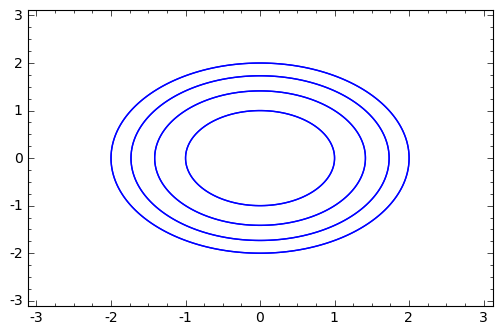
\includegraphics[width=8cm]{pictures_bitmap/niveauCercles.png}
\end{center}
Notez que les courbes sont censées être des cercles : les axes $X$ et $Y$ n'ont pas la même échelle. 

%Vous trouverez sur \href{http://www.sagenb.org/home/pub/23/}{cette page} tout ce qu'il vous faudra pour créer des courbes de niveau avec Sage.
%TODO : cette adresse n'est plus valide. Il faut retrouver où elle est passés sur sagemath.org (sagenb est devenu sagemath)

\begin{example}
    Un exemple plus riche en enseignements est celui de la fonction
    \begin{equation}
        f(x,y)=x^2-y^2.
    \end{equation}
    La courbe de niveau $h$ est donnée par l'équation $x^2-y^2=h$.

    Commençons par $h=0$. Dans ce cas nous avons $(x+y)(x-y)=0$ et par conséquent les courbes de niveau de hauteur zéro sont les deux droites $x+y=0$ et $x-y=0$.

    Voyons ensuite la courbe de niveau $h=1$. Cela est l'équation $x^2-y^2=1$, c'est à dire
    \begin{equation}
        y(x)=\pm\sqrt{x^2-1}.
    \end{equation}
    C'est une fonction qui n'est définie que pour $| x |\geq 1$. Avec $x=1$ nous avons $y=1$. Ensuite, lorsque $x$ grandit, $y$ grandit également, mais la courbe ne peut pas croiser la courbe de niveau $h=0$. Donc, suivant les notations de la figure \ref{LabelFigCQIXooBEDnfK}, la courbe de niveau «part» de $P$ et doit monter sans croiser les diagonales.

 % les figures CQIXooBEDnfK et KGQXooZFNVnW sont générées par le script MBFDooRFPyNW

%The result is on figure \ref{LabelFigCQIXooBEDnfK}. % From file CQIXooBEDnfK
\newcommand{\CaptionFigCQIXooBEDnfK}{La courbe de niveau $h=1$ de $x^2-y^2$. Notez qu'elle est en deux morceaux.}
\input{auto/pictures_tex/Fig_CQIXooBEDnfK.pstricks}

%The result is on figure \ref{LabelFigKGQXooZFNVnW}. % From file KGQXooZFNVnW
\newcommand{\CaptionFigKGQXooZFNVnW}{La courbe de niveau $x^2-y^2=-1$.}
\input{auto/pictures_tex/Fig_KGQXooZFNVnW.pstricks}

    En ce qui concerne la courbe de niveau $h=-1$, elle correspond à la courbe $y=\pm\sqrt{1+x^2}$ qui est définie pour tous les $x\in\eR$. Le même raisonnement que précédemment nous amène à la figure \ref{LabelFigKGQXooZFNVnW}.

\end{example}

Une autre façon de voir les courbe de niveau est de dire que la courbe de niveau de hauteur $h$ est la projection dans le plan $XY$ de la section du graphe de $f$ par le plan $z=h$.

On peut également définir le graphe de fonctions de trois (ou plus) variables. Le graphe de la fonction $f\colon D\subset\eR^3\to \eR$ est l'ensemble
\begin{equation}
    \big\{ \big( x,y,z,f(x,y,z) \big)\tq (x,y,z)\in D \big\}\subset \eR^4.
\end{equation}
De tels graphes ne peuvent pas être représentés sur une feuille de papier. Il est toutefois possible de définir les ensembles de niveaux :
\begin{equation}
    E_h=\big\{ (x,y,z)\in D\tq  f(x,y,z)=h\big\}.
\end{equation}
Ce sont des surfaces dans $\eR^3$ que l'on peut dessiner.

\begin{example}
    Les surfaces de niveau de la fonction $f(x,y,z)=x^2+y^2+z^2$ sont des sphères. Il n'y a pas de surfaces de niveau pour les «hauteurs» négatives.
\end{example}

\begin{example}
    Considérons la fonction $f(x,y,z)=x^2+y^2-z^2$. En coordonnées cylindrique, cette fonction s'écrit
    \begin{equation}
        f(r,\theta,z)=r^2-z^2.
    \end{equation}
    La surface de niveau $0$ est donnée par l'équation $r=| z |$. Cela fait un cercle à chaque hauteur, dont le rayon grandit linéairement avec la hauteur; le tout est donc un cône. C'est d'ailleurs le cône obtenu par rotation de la courbe de niveau $h=0$ que nous avions obtenue pour la fonction $x^2-y^2$.

    En ce qui concerne les ensembles de niveau positifs, ils sont donnés par
    \begin{equation}
        z=\pm\sqrt{x^2+y^2-h}.
    \end{equation}
    Notez qu'ils ne sont pas définis pour $r\geq h$. Cela pose un petit problème quand on veut le tracer à l'ordinateur :
    \begin{verbatim}
----------------------------------------------------------------------
| Sage Version 4.6.1, Release Date: 2011-01-11                       |
| Type notebook() for the GUI, and license() for information.        |
----------------------------------------------------------------------
sage: var('x,y')
(x, y)
sage: f(x,y)=sqrt(x**2+y**2-3)
sage: F=plot3d(f(x,y),(x,-5,5),(y,-5,5)) 
sage: G=plot3d(-f(x,y),(x,-5,5),(y,-5,5))    
sage: F+G
    \end{verbatim}
Le résultat est\footnote{Encore une fois : ça donne mieux à l'écran, et vous pouvez le faire bouger; je vous encourage à le faire !} :
    \begin{center}
            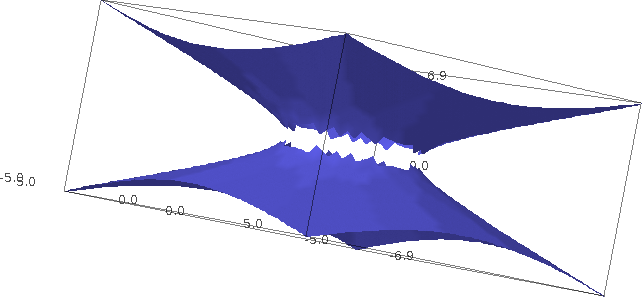
\includegraphics[width=15cm]{pictures_bitmap/AdSmauvais.png}
    \end{center}
    On voit qu'il y a un grand trou au centre correspondant aux $z$ proches de zéro. Or d'après l'équation, il n'en est rien : en $z=0$ il y a bel et bien tout un cercle. Afin d'obtenir une meilleur image, il faut demander de tracer avec un maillage plus fin :
    \begin{verbatim}
----------------------------------------------------------------------
| Sage Version 4.6.1, Release Date: 2011-01-11                       |
| Type notebook() for the GUI, and license() for information.        |
----------------------------------------------------------------------
sage: var('x,y')
(x, y)
sage: f(x,y)=sqrt(x**2+y**2-3)
sage: F=plot3d(f(x,y),(x,-5,5),(y,-5,5),plot_points=300) 
sage: G=plot3d(-f(x,y),(x,-5,5),(y,-5,5),plot_points=300)
sage: F+G
    \end{verbatim}
    Le temps de calcul est un peu plus long, mais le résultat est meilleur :
    \begin{center}
            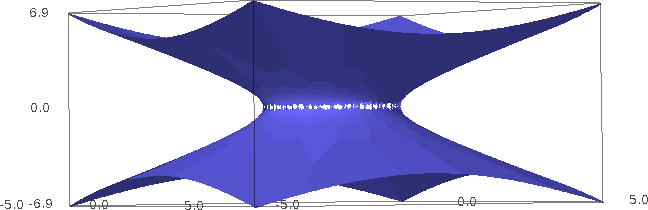
\includegraphics[width=15cm]{pictures_bitmap/AdSbon.png}
    \end{center}
\end{example}

%+++++++++++++++++++++++++++++++++++++++++++++++++++++++++++++++++++++++++++++++++++++++++++++++++++++++++++++++++++++++++++
%\section{Calcul de limites}
%+++++++++++++++++++++++++++++++++++++++++++++++++++++++++++++++++++++++++++++++++++++++++++++++++++++++++++++++++++++++++++

%Incidemment, le lemme \ref{Def_diff2} nous donne une nouvelle technique pour calculer des limites à plusieurs variables, similaire à celle du développement asymptotique expliquée dans la section \ref{SecTaylorR}.

%En effet, la formule \eqref{def_diff2} nous permet d'écrire $f(x)$ sous la forme
%\begin{equation}
%	f(x)=f(a)+df(a).(x-a)+\sigma_f(a,x)\| x-a \|
%\end{equation}
%où la fonction $\sigma_f$ satisfait $\lim_{x\to a}\sigma_f(a,x)=0$. Ici, $x$ et $a$ sont des éléments de $\eR^m$.

%++++++++++++++++++++++++++++++++++++++++++++++++++++++++++++++++++++++++++++++++++++++++
\section{Fonctions de classe $\mathcal{C}^1$}
%++++++++++++++++++++++++++++++++++++++++++++++++++++++++++++++++++++++++++++++++++++++++++++++++++++++++++++++++++++++++++++++

Soit $f$ une fonction différentiable de $U$, ouvert de $\eR^m$, dans $\eR^n$. L'application différentielle de $f$ est une application  de $\eR^m$ dans $\mathcal{L}(\eR^m, \eR^n)$ 
\begin{equation}
  \begin{array}{rccc}
    df : & \eR^m & \to & \mathcal{L}(\eR^m, \eR^n)\\
& a& \mapsto & df_a.
  \end{array}
\end{equation}
Nous savons que $\mathcal{L}(\eR^m, \eR^n)$ est un espace vectoriel normé avec la définition \ref{DefDQRooVGbzSm}. Si $T$ est un élément dans $\mathcal{L}(\eR^m, \eR^n)$ alors la norme de $T$ est définie par 
\[
\|T\|_{\mathcal{L}(\eR^m, \eR^n)}=\sup_{x\in\eR^m} \frac{\|T(x)\|_n}{\|x\|_m}=\sup_{\begin{subarray}{l}
    x\in\eR^m\\
\|x\|_m\leq 1
  \end{subarray}} \|T(x)\|_n.
\]

Lorsqu'il existe un $M>0$ tel que $\| df(a) \|_{\aL(\eR^m,\eR^n)}<M$ pour tout $a$ dans $U$, nous disons que la différentielle de $f$ est \defe{bornée}{bornée!différentielle} sur $U$.

\begin{definition}
	La fonction $f$ est dite \defe{de classe $\mathcal{C}^1$}{fonction!de classe  $\mathcal{C}^1$} de $U\subset\eR^m$  dans $\eR^n$ si son application différentielle $df$ est continue de $\eR^m$ dans $\mathcal{L}(\eR^m, \eR^n)$. Nous écrivons $f\in\mathcal{C}^1(U,\eR^n)$\nomenclature{$\aC^1(U,\eR^n)$}{Les applications une fois continument dérivables}.
\end{definition}

\begin{proposition}		\label{PropDerContCun}
	Une fonction \( f\colon U\to \eR^n\) où \( U\) est ouvert dans \( \eR^m\) est de classe \( C^1\) si et seulement si les dérivées partielles de $f$ existent et sont continues.
\end{proposition}

\begin{proof}
	Supposons que les dérivées partielles de $f$ existent et sont continues. Nous savons alors déjà par la proposition \ref{Diff_totale} que la fonction $f$ est différentiable et qu'elle s'exprime sous la forme
	\[
		df_a(h)=\sum_{i=1}^{m}\partial_if (a)h_i, \qquad \forall a \in U,\,\forall h\in\eR^m.
	\]
	Pour montrer que $df$ est continue, nous devons montrer que la quantité $\| df(x)-df(a) \|_{\aL(\eR^m,\eR^n)}$ peut être rendue arbitrairement petite si $\| x-a \|_m$ est rendu petit. Nous avons
	\begin{equation}
		\begin{aligned}
			\| df_x-df_a \|_{\aL}&=\sup_{\| h \|=1}\| df_x(h)-df_a(h) \|\\
			&=\sup_{\| h \|_m=1}\left\|\sum_{i=1}^{m}\left(\partial_if (x)-\partial_if (a)\right)h_i\right\|_n\leq\\
			&\leq\sup_{\| h \|_m=1}\sum_{i=1}^{m} \left\|\left(\partial_if (x)-\partial_if (a)\right)\right\|_n|h_i|\leq\\
			&\leq\sup_{\| h \|_m=1} \|h\|_\infty\sum_{i=1}^{m} \left\|\left(\partial_if (x)-\partial_if (a)\right)\right\|_n\\
			&\leq \sum_{i=1}^m\| \partial_if(x)-\partial_if(a) \|.
		\end{aligned}
	\end{equation}
	Dans ce calcul, nous avons utilisé le fait que si $\| h \|_m\leq 1$, alors $\| h \|_{\infty}\leq 1$. Étant donné la continuité de $\partial_if$, la dernière ligne peut être rendue arbitrairement petite lorsque $x$ est proche e $a$.

Supposons maintenant que $f$ soit dans $\mathcal{C}^1(U,\eR^n)$. Alors 
\[
\left\|\partial_if (x)-\partial_if (a)\right\|_n= \left\|df(x).e_i-df(a).e_i\right\|_n \leq  \left\|df(x)-df(a)\right\|_{\mathcal{L}(\eR^m,\eR^n)},
\]  
la continuité de $df$ implique donc celle de $\partial_i f$ pour tout $i$ dans $\{1,\ldots,m\}$.
\end{proof}
\begin{proposition}
  Soient $U$ un ouvert de $\eR^m$ et $V$ un ouvert de $\eR^n$. Soient $f: U\to V$  dans $\mathcal{C}^1(U,V)$ et $g: V \to \eR^p$ dans $\mathcal{C}^1(V,\eR^n)$.  Alors la fonction composée $g\circ f: U\to \eR^p $ est dans $\mathcal{C}^1(U,\eR^p)$.
\end{proposition}
\begin{proof} On fixe $a$ dans $U$ 
  \begin{equation}
    \begin{aligned}
     \big\|d(g\circ f)(x)&-d(g\circ f)(a)\big\|_{\mathcal{L}(\eR^m,\eR^p)}\\
     &=\left\|dg(f(x))\circ df(x)-dg(f(a))\circ df(a)\right\|_{\mathcal{L}(\eR^m,\eR^p)}\leq\\
&\leq \left\|\left(dg(f(x))-dg(f(a))\right)\circ df(x)\right\|_{\mathcal{L}(\eR^m,\eR^p)}+\\
&\quad+ \left\|dg(f(a))\circ \left(df(x)-df(a)\right)\right\|_{\mathcal{L}(\eR^m,\eR^p)}\leq\\
&\leq \left\|dg(f(x))-dg(f(a))\right\|_{\mathcal{L}(\eR^n,\eR^p)}\left\| df(x)\right\|_{\mathcal{L}(\eR^m,\eR^n)}+\\
&\quad+ \left\|dg(f(a))\right\|_{\mathcal{L}(\eR^n,\eR^p)}\left\| df(x)-df(a)\right\|_{\mathcal{L}(\eR^n,\eR^p)}.\\
    \end{aligned}
  \end{equation}
On peut conclure en passant à la limite $x\to a$ parce que les fonctions $f$, $g$, $df$ et $dg$ sont continues, de telle sorte que
\begin{equation}
	\begin{aligned}[]
		\lim_{x\to a} dg\big( f(x) \big)=dg\big( f(a) \big)\\
		\lim_{x\to a} df(x)=df(a).
	\end{aligned}
\end{equation}
\end{proof}

\begin{remark}
  On peut prouver le même résultat en utilisant la continuité de l'application bilinéaire 
\begin{equation}
  \begin{array}{rccc}
    \circ : & \mathcal{C}^1(U,V)\times\mathcal{C}^1(V,\eR^p)  & \to & \mathcal{L}(U, \eR^p)\\
& (T,S)& \mapsto & T\circ S.
  \end{array}
\end{equation}
\end{remark}
%+++++++++++++++++++++++++++++++++++++++++++++++++++++++++++++++++++++++++++++++++++++++++++++++++++++++++++++++++++++++++++
\section{Dérivée directionnelle de fonctions composées}		\label{SecDerDirFnComp}
%+++++++++++++++++++++++++++++++++++++++++++++++++++++++++++++++++++++++++++++++++++++++++++++++++++++++++++++++++++++++++++

Étant donné que nous allons voir en détail la différentielle de fonctions composées à la proposition \ref{PropDiffCompose}, nous n'allons pas rentrer dans tous les détail ici.

Nous savons déjà comment dériver les fonctions composées de $\eR$ dans $\eR$. Si nous avons deux fonctions $f\colon \eR\to \eR$ et $u\colon \eR\to \eR$, nous formons la composée $\varphi=f\circ u\colon \eR\to \eR$ dont la dérivée vaut
\begin{equation}
	\varphi'(a)=f'\big( u(a) \big)u'(a).
\end{equation}

Considérons maintenant le cas un peu plus compliqué des fonctions $f\colon \eR\to \eR$ et $u\colon \eR^2\to \eR$, et de la composée
\begin{equation}
	\begin{aligned}
		\varphi\colon \eR^2&\to \eR \\
		\varphi(x,y)&= f\big( u(x,y) \big). 
	\end{aligned}
\end{equation}
Afin de calculer la dérivée partielle de $\varphi$ par rapport à $x$, nous admettons que pour tout $a$, $b$ et $t$, il existe $c\in\mathopen[ a , a+t \mathclose]$ tel que
\begin{equation}
	u(a+t,b)=u(a,b)+t\frac{ \partial u }{ \partial x }(c,b).
\end{equation}
Cela est une généralisation immédiate du théorème \ref{ThoAccFinis}. Nous devons calculer
\begin{equation}		\label{EqPremPasDiffxvp}
	\frac{ \partial \varphi }{ \partial x }(a,b)=\lim_{t\to 0} \frac{ \varphi(a+t,b)-\varphi(a,b) }{ t }=\lim_{t\to 0} \frac{ f\big( u(a+t,b) \big)-g\big( u(a,b) \big) }{ t }.
\end{equation}
Étant donné l'hypothèse que nous avons faite sur $u$, nous avons
\begin{equation}
	f\big( u(a+t,b) \big)=f\big( u(a,b)+t\frac{ \partial u }{ \partial x }(c,b) \big).
\end{equation}
En utilisant le théorème des accroissements finis pour $f$, nous avons un point $d$ entre $u(a,b)$ et $u(a,b)+t\frac{ \partial u }{ \partial x }(c,b)$ tel que
\begin{equation}
	f\big( u(a,b)+t\frac{ \partial u }{ \partial x }(c,b) \big)=f\big( u(a,b) \big)+t\frac{ \partial u }{ \partial x }(c,b)f'(d).
\end{equation}
Le numérateur de \eqref{EqPremPasDiffxvp} devient donc
\begin{equation}
	t\frac{ \partial u }{ \partial x }(c,b)f'(d).
\end{equation}
Certes les points $c$ et $d$ sont inconnus, mais nous savons que $c$ est entre $a$ et $a+t$ ainsi que $d$ se situe entre $u(a,b)$ et $u(a,b)+t\frac{ \partial u }{ \partial x }(c,b)$. Lorsque nous prenons la limite $t\to 0$, nous avons donc $\lim_{t\to 0} c=a$ et $\lim_{t\to 0} d=u(a,b)$. Nous avons alors
\begin{equation}
	\lim_{t\to 0} \frac{ t\frac{ \partial u }{ \partial x }(c,b)f'(d) }{ t }=\frac{ \partial u }{ \partial x }(a,b)f'\big( u(a,b) \big).
\end{equation}
La formule que nous avons obtenue (de façon pas très rigoureuse) est
\begin{equation}
	\frac{ \partial  }{ \partial x }f\big( u(x,y) \big)=\frac{ \partial u }{ \partial x }(x,y)f'\big( u(x,y) \big).
\end{equation}

Prenons maintenant un cas un peu plus compliqué où nous voudrions savoir les dérivées partielles de la fonction $\varphi$ donnée par
\begin{equation}
	\varphi(x,y,z)=f\big( u(x,y),v(x,y,z) \big)
\end{equation}
où $f\colon \eR^2\to \eR$, $u\colon \eR^2\to \eR$ et $v\colon \eR^3\to \eR$. 

Commençons par la dérivée partielles par rapport à $z$. Étant donné que $\varphi$ ne dépend de $z$ que via la seconde entrée de $f$, il est normal que seule la dérivée partielle de $f$ par rapport à sa seconde entrée arrive dans la formule :
\begin{equation}
	\frac{ \partial \varphi }{ \partial z }(x,y,z)=\frac{ \partial f }{ \partial v }\big( u(x,y),v(x,y,z) \big)\frac{ \partial v }{ \partial z }(x,y,z).
\end{equation}
La dérivée partielle par rapport à $y$ demande de tenir compte en même temps de la façon dont $f$ varie avec sa première entrée et la façon dont elle varie avec sa seconde entrée; cela nous fait deux termes :
\begin{equation}
	\frac{ \partial \varphi }{ \partial y }(x,y,z)=\frac{ \partial f }{ \partial u }\big( u(x,y),v(x,y,z) \big)\frac{ \partial u }{ \partial y }(x,y)+\frac{ \partial f }{ \partial v }\big( u(x,y),v(x,y,z) \big)\frac{ \partial v }{ \partial y }(x,y,z).
\end{equation}


Cette formule a une interprétation simple. Lançons un caillou du sommet d'une falaise. Son mouvement est une chute libre avec une vitesse initiale horizontale :
\begin{subequations}
	\begin{numcases}{}
		x(t)=v_0t\\
		y(t)=h_0-\frac{ gt^2 }{ 2 }
	\end{numcases}
\end{subequations}
où $v_0$ est la vitesse initiale horizontale et $h_0$ est la hauteur de la falaise. Si nous sommes intéressés à la distance entre le caillou et le bas de la falaise (point $(0,0)$), le théorème de Pythagore nous dit que
\begin{equation}
	d(t)=\sqrt{x^2(t),y^2(t)}.
\end{equation}
Pour trouver la variation de la distance par rapport au temps il faut savoir de combien la distance varie lorsque $x$ varie et multiplier par la variation de $x$ par rapport à $t$, et puis faire la même chose avec $y$.

\begin{theorem}		\label{ThoDerDirFnComp}
	Soit $g\colon \eR^m\to \eR^n$ une fonction différentiable en $a$, et $f\colon \eR^n\to \eR^p$ une fonction différentiable en $g(a)$. Si nous définissons $\varphi(x)=(f\circ g)(x)$, alors pour tout $i=1,\ldots,m$, nous avons
	\begin{equation}
		\frac{ \partial \varphi }{ \partial x_i }(a)=\sum_{k=1}^n\frac{ \partial f }{ \partial y_k }\big( g(a) \big)\frac{ \partial g }{ \partial x_i }
	\end{equation}
	où $\frac{ \partial f }{ \partial y_k }$ dénote la dérivée partielle de $f$ par rapport à sa $k$-ième variable.
\end{theorem}

Donnons un exemple d'utilisation de cette formule. Si
\begin{equation}
	\begin{aligned}[]
		g\colon \eR^2\to \eR^3\\
		f\colon \eR^3\to \eR,
	\end{aligned}
\end{equation}
nous avons $\varphi\colon \eR^2\to \eR$. Les dérivées partielles de $\varphi$ sont données par les formules
\begin{equation}
	\frac{ \partial \varphi }{ \partial x }(x,y)=\frac{ \partial f }{ \partial x_1 }\big( g(x,y) \big)\frac{ \partial g_1 }{ \partial x }(x,y)+\frac{ \partial f }{ \partial x_2 }\big( g(x,y) \big)\frac{ \partial g_2 }{ \partial y }(x,y)+\frac{ \partial f }{ \partial x_3 }\big( g(x,y) \big)\frac{ \partial g_3 }{ \partial x }(x,y)
\end{equation}
et
\begin{equation}
	\frac{ \partial \varphi }{ \partial y }(x,y)=\frac{ \partial f }{ \partial x_1 }\big( g(x,y) \big)\frac{ \partial g_1 }{ \partial y }(x,y)+\frac{ \partial f }{ \partial x_2 }\big( g(x,y) \big)\frac{ \partial g_2 }{ \partial y }(x,y)+\frac{ \partial f }{ \partial x_3 }\big( g(x,y) \big)\frac{ \partial g_3 }{ \partial y }(x,y)
\end{equation}
Notez que les dérivées de $\varphi$ et des composantes de $g$ sont calculées en $(x,y)$, tandis que celles de $f$ sont calculées en $g(x,y)$.

%++++++++++++++++++++++++++++++++++++++++++++++++++++++++++++++++++++++++++++++++++++++++++++++++++++++++++++++++++++++
\section{Théorèmes des accroissements finis}		\label{SecThoAccrsFinis}
%++++++++++++++++++++++++++++++++++++++++++++++++++++++++++++++++++++++++++++++++++++++++++++++++++++++++++++++++++++++

Nous avons déjà démontré (lemme \ref{LemdfaSurLesPartielles}) que si $f$ est différentiable au point $x$ alors  $df_x(u)=\partial_uf(x)$. Une importante conséquence est le théorème des accroissements finis
\begin{theorem}[Accroissements finis, inégalité de la moyenne]\label{val_medio_2}
   Soit $U$ un ouvert dans $\eR^m$ et soit $f:U\to\eR^n$ une fonction différentiable. Soient $a$ et $b$ deux point dans $U$, $a\neq b$, tels que le segment $[a,b]$ soit contenu dans $U$. Alors
   \begin{equation}
        \|f(b)-f(a)\|_n\leq \sup_{x\in[a,b]}\|df(x)\|_{\mathcal{L}(\eR^m,\eR^n)}\|b-a\|_m.
   \end{equation}
\end{theorem}
\index{application!différentiable}
\index{inégalité!de la moyenne}
\index{théorème!accroissements finis!forme générale}

\begin{proof}
 On utilise le théorème \ref{val_medio_1} et le fait que 
\[
\|\partial_u f(x)\|_n\leq \|df(x)\|_{\mathcal{L}(\eR^m,\eR^n)}\|u\|_m,
\]
pour tout $u$ dans $\eR^m$.
\end{proof}

La proposition suivante est une application fondamentale du théorème des accroissements finis \ref{val_medio_2}.
\begin{proposition}		\label{PropAnnulationEtConstance}
	Soit $U$ un ouvert connexe par arcs de $\eR^m$ et une fonction $f\colon U\to \eR^n$. Les conditions suivantes sont équivalentes :
	\begin{enumerate}
		\item\label{ItemPropCstDiffZeroi}
			$f$ est constante;
		\item\label{ItemPropCstDiffZeroii}
			$f$ est différentiable et $df(a)=0$ pour tout $a\in U$;
		\item\label{ItemPropCstDiffZeroiii}
			les dérivées partielles $\partial_1f,\ldots,\partial_mf$ existent et sont nulles sur $U$.
	\end{enumerate}
\end{proposition}
\index{connexité!par arc!fonction différentiable}
\index{différentiabilité}

\begin{proof}
	Nous allons démonter les équivalences en plusieurs étapes. D'abord \ref{ItemPropCstDiffZeroi} $\Rightarrow$ \ref{ItemPropCstDiffZeroii}, puis \ref{ItemPropCstDiffZeroii} $\Rightarrow$ \ref{ItemPropCstDiffZeroiii}, ensuite \ref{ItemPropCstDiffZeroiii} $\Rightarrow$ \ref{ItemPropCstDiffZeroii} et enfin \ref{ItemPropCstDiffZeroii} $\Rightarrow$ \ref{ItemPropCstDiffZeroi}.

	Commençons par montrer que la condition \ref{ItemPropCstDiffZeroi} implique la condition \ref{ItemPropCstDiffZeroii}. Si $f(x)$ est constante, alors la condition \eqref{EqCritereDefDiff} est vite vérifiée en posant $T(h)=0$.

	Afin de voir que la condition \ref{ItemPropCstDiffZeroii} implique la condition \ref{ItemPropCstDiffZeroiii}, remarquons d'abord que la différentiabilité de $f$ implique que les dérivées partielles existent (proposition \ref{diff1}) et que nous avons l'égalité $df(a).u=\sum_iu_i\partial_if(a)$ pour tout $u\in\eR^m$ (lemme \ref{LemdfaSurLesPartielles}). L'annulation de $\sum_iu_i\partial_if(a)$ pour tout $u$ implique l'annulation des $\partial_if(a)$ pour tout $i$.

	Prouvons maintenant que la propriété \ref{ItemPropCstDiffZeroiii} implique la propriété \ref{ItemPropCstDiffZeroii}. D'abord, par la proposition \ref{Diff_totale}, l'existence et la continuité des dérivées partielles $\partial_if(a)$ implique la différentiabilité de $f$. Ensuite, la formule $df(a).u=\sum_i u_i\partial_if(a)$ implique que $df(a)=0$. 
	
	
	Il reste à montrer que \ref{ItemPropCstDiffZeroii} implique la condition \ref{ItemPropCstDiffZeroi}, c'est à dire que l'annulation de la différentielle implique la constance de la fonction. C'est ici que nous allons utiliser le théorème des accroissements finis. En effet, si $a$ et $b$ sont des points de $U$, le théorème \ref{val_medio_2} nous dit que
	\begin{equation}
		\|f(b)-f(a)\|_n\leq \sup_{x\in[a,b]}\|df(x)\|_{\mathcal{L}(\eR^m,\eR^n)}\|b-a\|_m.
	\end{equation}
	Mais $\| df(x) \|=0$ pour tout $x\in U$, donc ce supremum est nul et $f(b)=f(a)$, ce qui signifie la constance de la fonction.
\end{proof}

%\begin{proof}
%  \begin{itemize}
%  \item Le théorème \ref{val_medio_2} nous dit que si la différentielle de $f$ est nulle alors $f$ est constante sur chaque segment contenu dans $U$. Cela nous dit que $f$ est constante sur chaque boule contenue dans $U$, donc $f $ est localement constante. Il est possible de démontrer que toute fonction localement constante sur un connexe est constante.  
%\item Si toutes les dérivées partielles $\partial_1 f, \ldots, \partial_m f $ existents et sont identiquement nulles sur $U$ alors $f$ est différentiable et sa différentielle est identiquement nulle. On utilise la première partie de la preuve pour conclure. 
%  \end{itemize}
%\end{proof}

%+++++++++++++++++++++++++++++++++++++++++++++++++++++++++++++++++++++++++++++++++++++++++++++++++++++++++++++++++++++++++++
\section{Fonctions Lipschitziennes}
%+++++++++++++++++++++++++++++++++++++++++++++++++++++++++++++++++++++++++++++++++++++++++++++++++++++++++++++++++++++++++++


\begin{definition}      \label{DEFooQHVEooDbYKmz}
    Soient \( (E,d_E)\) et \( (F,d_F)\) deux espaces métriques\footnote{Pour rappel, les espaces métriques sont définis par la définition \ref{DefMVNVFsX} et le théorème \ref{ThoORdLYUu}; je précise que nous ne supposons pas que \( E\) soit vectoriel; en particulier il peut être un ouvert de \( \eR^n\).}, \( f\colon E\to F\) une application et un réel \( k\) strictement positif. Nous disons que \( f\) est \defe{Lipschitzienne}{Lipschitzienne} de constante $k$ sur \( E\) si pour tout \( x,y\in E\),
    \begin{equation}
        d_F\big( f(x)-f(y) \big)\leq kd_E(x,y).
    \end{equation}
\end{definition}
%TODO : faire la chasse aux endroits où cette définition devrait être référencée.
Soit \( f\) une fonction \( k\)-Lipschitzienne. Si \( y\in \overline{ B(x,\delta)}\) alors \( \| x-y \|\leq\delta\) et donc \( \big\| f(x)-f(y) \big\|\leq k\delta\). Cela signifie que la condition Lipschitz pour s'énoncer en termes de boules fermées par
\begin{equation}    \label{EqDZvtUbn}
    f\big( \overline{ B(x,\delta) } \big)\subset \overline{  B\big( f(x),k\delta \big) }
\end{equation}
tant que \( \overline{ B(x,\delta) } \) est contenue dans le domaine sur lequel \( f\) est Lipschitz.

\begin{proposition}
  Soit  $U$ un ouvert convexe  de $\eR^m$, et soit $f:U\to \eR^n$ une fonction différentiable. La fonction $f$ est Lipschitzienne sur $U$ si et seulement si $df$ est bornée sur $U$.  
\end{proposition}
\begin{proof}
	Le fait que l'application différentielle $df$ soit bornée signifie qu'il existe un $M>0$ dans $\eR$ tel que $\|df_a\|_{\mathcal{L}(\eR^m,\eR^n)}\leq M$, pour tout $a$ dans $U$. Si cela est le cas, alors le théorème \ref{val_medio_2} et la convexité\footnote{La convexité de $U$ sert à assurer que la droite reliant $a$ à $b$ est contenue dans $U$; c'est ce que nous utilisons dans la démonstration du théorème \ref{val_medio_2}.} de $U$ impliquent évidemment que $f$ est de Lipschitz de constante plus petite ou égale à $M$.
	
	Inversement, si $f$ est Lipschitz de constante $k$, alors pour tout $a$ dans $U$ et $u$ dans $\eR^m$ on a 
	\[
		\left\|\frac{f(a+tu)-f(a)}{t}\right\|_n\leq k \|u\|_m,
	\]   
	En passant à la limite pour $t\to 0$ on a 
	\[
		\|\partial_u f(a)\|_n=\|df_a(u)\|_n\leq k \|u\|_m,
	\]
	donc la norme de $df_a$ est majorée par $k$ pour tout $a$ dans $U$.   
\end{proof}

Notez cependant qu'une fonction peut être Lipschitzienne sans être différentiable.

\begin{proposition} \label{PropFZgFTEW}
    Une fonction Lipschitzienne \( f\colon \eR\to \eR\) est continue.
\end{proposition}

\begin{proof}
    Nous utilisons la caractérisation de la continuité donnée par le théorème \ref{ThoESCaraB}. Prouvons donc la continuité en \( a\in \eR\). Pour tout \( x\) nous avons
    \begin{equation}
        \big| f(x)-f(a) \big|\leq k| x-a |.
    \end{equation}
    Si \( \epsilon>0\) est donné, il suffit de prendre \( \delta<\frac{ \epsilon }{ k }\) pour avoir
    \begin{equation}
        \big| f(x)-f(a) \big|\leq k\frac{ \epsilon }{ k }=\epsilon.
    \end{equation}
    Donc \( f\) est continue en \( a\).
\end{proof}

\begin{definition}      \label{DefJSFFooEOCogV}
    Une fonction 
    \begin{equation}
        \begin{aligned}
            f\colon \eR^n\times \eR^m&\to \eR^p \\
            (t,y)&\mapsto f(t,y) 
        \end{aligned}
    \end{equation}
    est \defe{localement Lipschitz}{Lipschitz!localement} en \( y\) au point \( (t_0,y_0)\) s'il existe des voisinages \( V\) de \( t_0\) et \( W\) de \( y_0\) et un nombre \( k>0\) tels que pour tout \( (t,y)\in V\times W\) on ait
    \begin{equation}
        \big\| f(t_0,y_0)-f(t,y) \big\|\leq k\| y-y_0 \|.
    \end{equation}
    La fonction est localement Lipschitz sur un ouvert \( U\) de \( \eR^n\times \eR^m\) si elle est localement Lipschitz en chaque point de \( U\).
\end{definition}

\begin{normaltext}      \label{NORMooYNRAooBgobcK}
    Autrement dit, une fonction est localement Lipschitzienne en sa deuxième variable lorsque tout point admet un voisinage sur lequel elle est Lipschitzienne.
\end{normaltext}

\begin{proposition}     \label{PropGIBZooVsIqfY}
    Si \( f\) et \( g\) sont deux fonctions localement Lipschitz alors \( f+g\) l'est.
\end{proposition}

\begin{proof}
    Il s'agit d'un simple calcul avec une majoration standard :
    \begin{subequations}
        \begin{align}
            \| (f+g)(t_0,y_0)-(f+g)(t,y) \|&\leq \|  f(t_0,y_0)-f(t,y)  \|+\| g(t_0,y_0)-g(t,y) \|\\
            &\leq k_f\| y-y_0 \|+k_g\| y-y_0 \|\\
            &=(k_f+k_g)\| y-y_0 \|.
        \end{align}
    \end{subequations}
\end{proof}

\begin{lemma}   \label{LemCFZUooVqZmpc}
    La fonction donné par
    \begin{equation}
        f(t, (x,y) )=xy
    \end{equation}
    est localement Lipschitz en tout point.
\end{lemma}

\begin{proof}
    Nous avons la majoration classique
    \begin{equation}
        | f\big(t,(x_0,y_0)\big)-f\big( t,(x,y) \big) |=| x_0y_0-xy |\leq| x_0y_0-x_0y |+| x_0y-xy |\leq | x_0 || y_0-y |+| y || x_0-x |.
    \end{equation}
    Vu que nous parlons de fonction \emph{localement Lipschitzienne}, nous pouvons majorer \( | y |\) et \( | x_0 |\) par un même nombre \( k\) dans un voisinage de \( (x_0,y_0)\). Cela donne
    \begin{equation}
        | f\big(t,(x_0,y_0)\big)-f\big( t,(x,y) \big) |\leq k\big( | y_0-y |+| x_0-x | \big)\leq \sqrt{2}k\| \begin{pmatrix}
            x_0-x    \\ 
            y_0-y    
        \end{pmatrix}\|.
    \end{equation}
    Nous avons utilisé l'équivalence de norme de la proposition \ref{PropLJEJooMOWPNi}\ref{ItemABSGooQODmLNi}.
\end{proof}



%++++++++++++++++++++++++++++++++++++++++++++++++++++++++++++++++++++++++++++++++++++++++
\section{Différentielles d'ordre supérieur}		\label{SecDiffOrdSup}
%++++++++++++++++++++++++++++++++++++++++++++++++++++++++++++++++++++++++++++++++++++++++++++++++++++++++++++++++++++++++++++++
\begin{definition}
	Soit $U$ un ouvert de $\eR^m$ et  $f:U\subset\eR^m\to \eR^n$ une fonction. La fonction $f$ est dite \defe{deux fois différentiable}{différentiable!deux fois} au point $a$ dans $U$,  si $f$ est différentiable dans un voisinage de $a$, et sa différentielle $df$ est différentiable au point $a$ en tant que application de $U$ dans $\mathcal{L}(\eR^m, \eR^n)$.  

La fonction $f$ sera dite deux fois différentiable sur l'ensemble $U$ si elle est deux fois différentiable en chaque point de $U$.

\end{definition}

%--------------------------------------------------------------------------------------------------------------------------- 
\subsection{Identification des espaces d'applications multilinéaires}
%---------------------------------------------------------------------------------------------------------------------------

La différentielle de la différentielle de $f$ est notée 
\[
d(df)(a)=d^2f(a),
\]
et est une application de $U$ dans $\mathcal{L}(\eR^m,\mathcal{L}(\eR^m, \eR^n) )$. Comme on a vu dans la proposition \ref{isom_isom}, l'espace $\mathcal{L}(\eR^m,\mathcal{L}(\eR^m, \eR^n) )$ est isométriquement isomorphe à l'espace $\mathcal{L}(\eR^m\times\eR^m, \eR^n )$. On verra comment cette propriété  est utilisé dans l'exemple \ref{bilin_2diff}.


Soient \( V\) et \( W\) deux espace vectoriel normés de dimension finie et \( \mO\) un ouvert autour de \( x\in V\). D'une part l'espace des applications linéaires \( \aL(V,W)\) est lui-même un espace vectoriel normé de dimension finie, et on peut identifier \(  \aL\big( V,\aL^{(k)}(V,W) \big)\)\nomenclature[Y]{\( \aL^{(n)}(V,W)\)}{L'espace des applications \( n\)-linéaires \( V^n\to W\)} avec \( \aL^{(k+1)}(V,W)\), ce qui nous permet de dire que la \( k\)\ieme\ différentielle est une application
\begin{equation}
    d^kf\colon \mO\to \aL^{(k)}(V,W).
\end{equation}
Plus précisément, l'identification se fait de la façon suivante : si \( \omega\in \aL\big( V,\aL^{(k)}(V,W) \big)\), alors \( \omega\) vu dans \( \aL^{(k+1)}(V,W)\) est définie par
\begin{equation}
    \omega(u_1,\ldots, u_{k+1})=\omega(u_1)(u_2,\ldots, u_{k+1}).    
\end{equation}

Cela étant posé nous pouvons donner les définition.

%--------------------------------------------------------------------------------------------------------------------------- 
\subsection{Fonctions différentiables plusieurs fois}
%---------------------------------------------------------------------------------------------------------------------------

\begin{definition}  \label{DefPNjMGqy}
    La fonction \( f\colon \mO\subset V\to W\) est
    \begin{enumerate}
        \item
            de classe \( C^0\) si elle est continue,
        \item
            de classe \( C^1\) si \( df\colon \mO\to \aL(V,W)\) est continue,
        \item
            de classe \( C^k\) si \( d^kf\colon \mO\to \aL^{(k)}(V,W)\) est continue,
        \item
            de classe \(  C^{\infty}\) si \( f\) est dans \( \bigcap_{k=0}^{\infty}C^k(V,W)\).
    \end{enumerate}
\end{definition}
\index{application!différentiable}
\index{application!de classe \( C^k\)}

\begin{definition}
    Un \defe{\( C^k\)-difféomorphisme}{difféomorphisme!de classe $C^k$} est une application inversible de classe \( C^k\) dont l'inverse est également de classe \( C^k\).
\end{definition}

\begin{example}\label{bilin_2diff}
	Soit $B:\eR^m\times \eR^m\to\eR^n$ une application bilinéaire. On définit $f:\eR^m\to\eR^n$ par $f(x)=B(x,x)$. Le lemme \ref{bilin_diff} nous dit que $B$ est différentiable. Cela implique la différentiabilité de $f$. Pour trouver la différentielle de la fonction $f$, nous écrivons $f=B\circ s$ où $s\colon \eR^m\to \eR^m\times\eR^m$ est l'application $s(x)=(x,x)$. En utilisant la règle de différentiation de fonctions composées,
	\begin{equation}
		df(a)=dB\big( s(a) \big)\circ ds(a).
	\end{equation}
	Mais $ds(a).u=(u,u)$ parce que $s(a+h)-s(a)-(h,h)=0$. Par conséquent,
	\begin{equation}		\label{EqdBsaExp}
		df(a).u=dB\big( s(a) \big)(u,u)=B(u,a)+B(a,u)
	\end{equation}
	où nous avons utilisé la formule du lemme \ref{bilin_diff}. La formule \eqref{EqdBsaExp} peut être écrite sous la forme compacte
	\begin{equation}
		df(a)=B(\cdot,a)+B(a,\cdot)
	\end{equation}
	La fonction $df(a)$ ainsi écrite est linéaire par rapport à $a$, donc différentiable. En outre elle coïncide avec sa différentielle, comme on a vu dans le remarque \ref{rk_lin}, au sens que la différentielle de $df$ au point $a$ sera l'application que à chaque $x$ dans $\eR^m$ associe l'application linéaire $B(x,\cdot)+B(\cdot, x)$. On voit bien que $d^2f$ au point $a$ est une application de $\eR^m$ vers l'espace des applications linéaires $\mathcal{L}(\eR^m, \eR^n)$. On peut utiliser d'autre part l'isomorphisme des espaces $\mathcal{L}(\eR^m,\mathcal{L}(\eR^m, \eR^n) )$ et $\mathcal{L}(\eR^m\times\eR^m, \eR^n )$ et dire que, une fois que $a$ est fixé, l'application $d^2f(a)$ est une application bilinéaire sur $\eR^m\times\eR^m$. On écrit alors $d^2f(a)(x,y)=B(x,y)+B(y,x)$.   
\end{example}

%--------------------------------------------------------------------------------------------------------------------------- 
\subsection{Différentielle seconde, fonction de classe \( C^2\)}
%---------------------------------------------------------------------------------------------------------------------------

Une condition nécessaire et suffisante pour l'existence de la différentielle seconde est la suivante
\begin{proposition}
   Soit $U$ un ouvert de $\eR^m$ et  $f:U\subset\eR^m\to \eR^n$ une fonction. La fonction $f$ est deux fois différentiable au point $a$ si et seulement si les dérivées partielles $\partial_1 f, \ldots, \partial_m f $ sont différentiables en $a$. 
\end{proposition}
Cela veut dire, en particulier, que $f$ est deux fois différentiable si et seulement si ses dérivées partielles secondes, $\partial_i\partial_j f$, pour toute couple d'indices $i,j$  dans $\{1,\ldots, m\}$, existent et sont continues. Pour les différentielles d'ordre supérieur on a la proposition suivante.

La différentielle seconde dans l'exemple  \ref{bilin_2diff} est symétrique, c'est à dire que $d^2f(a)(x_1,x_2)=d^2f(a)(x_2,x_1)$. En fait toute différentielle seconde est symétrique.  


\begin{theorem}[Schwarz]\label{Schwarz}
 Soit $U$ un ouvert de $\eR^m$ et  $f:U\subset\eR^m\to \eR^n$ une fonction de classe $\mathcal{C}^2$. Alors, pour toute couple $i,j$ d'indices dans $\{1,\ldots, m\}$ et pour tout point $a$ dans $U$, on a 
\[
\frac{\partial^2 f}{\partial  x_i\partial x_j}(a)=\frac{\partial^2 f}{\partial  x_j\partial x_i}(a).
\]
\end{theorem}
\begin{proof}
  Pour simplifier l'exposition nous nous limitons ici au cas $m=2$. Soit $(h,g)$ un vecteur fixé dans $\eR^2$. Pour tout  $v=(x,y)$ dans $\eR^2$ on note
  \begin{equation}
    \begin{array}{c}
      \Delta_h f(v)=f(v+he_1) -f(v) = f(x+h,y)-f(x,y),\\ 
      \Delta_g f(v)=f(v+ge_2) -f(v) = f(x,y+g)-f(x,y),\\ 
    \end{array}
  \end{equation}
Nous avons
\begin{equation}
  \begin{array}{c}
   \Delta_g   \Delta_h f(v)=\left(f(x+h,y+g)-f(x,y+g)\right)-\left(f(x+h,y)-f(x,y)\right),\\
   \Delta_h   \Delta_g f(v)=\left(f(x+h,y+g)-f(x+h,y)\right)-\left(f(x,y+g)-f(x,y)\right),
  \end{array}
\end{equation}
donc, 
\begin{equation}
  \frac{1}{g} \Delta_g  \left(\frac{1}{h} \Delta_h f(v)\right) = \frac{1}{h} \Delta_h \left(\frac{1}{g} \Delta_g f(v)\right).
\end{equation}
On utilise alors le théorème des accroissements finis
\[
\frac{1}{h} \Delta_h f(v)=\frac{1}{h}\big(f(x+h,y)-f(x,y)\big)=\frac{1}{h}\partial_1f(x+t_1h,y )h=\partial_1f(x+t_1h, y),
\]
pour un certain $t_1$ dans $]0,1[$. De même on obtient 
\[
\frac{1}{g} \Delta_g f(v)= \partial_2 f(x, y+t_2g),
\]
pour un certain $t_2$ dans $]0,1[$. Alors
 \begin{equation}
  \frac{1}{g} \Delta_g  \big(\partial_1f(x+t_1h, y)\big) = \frac{1}{h} \Delta_h \big(\partial_2 f(x, y+t_2g)\big).
\end{equation}
En appliquant encore une fois le théorème des accroissements finis on a
 \begin{equation}
  \partial_2\partial_1f(x+t_1h, y+s_1g) = \partial_1\partial_2 f(x+s_2h, y+t_2g).
\end{equation} 
Il suffit maintenant de passer à la limite pour $(h,g) \to (0,0)$ et de se souvenir du fait que $f$ est $\mathcal{C}^2$ seulement si ses dérivées partielles secondes sont continues pour avoir $\partial_2\partial_1f(v)=\partial_1\partial_2 f(v)$.
\end{proof}
Si $f$ est deux fois différentiable $d^2f(a)$ est l'application bilinéaire associée avec la matrice symétrique
\begin{equation}
 H_f(a)= \begin{pmatrix}
    \partial^2_1f(a)& \ldots& \partial_1\partial_m f(a)\\
    \vdots& \ddots& \vdots\\
    \partial_1\partial_m f(a)&\ldots&\partial^2_1f(a),
  \end{pmatrix}
\end{equation}
Cette matrice est dite la matrice \defe{hessienne}{hessienne} de $f$. 

\begin{example}
  Montrons qu'il n'existe pas de fonctions $f$ de classe $\mathcal{C}^2$ telles que 
  \begin{subequations}
      \begin{numcases}{}
  \partial_xf(x,y)= 5\sin x\\
  \partial_y(x,y)=6x+y.
      \end{numcases}
  \end{subequations}
  Ceci est vite fait en appliquant le théorème de Schwarz, \ref{Schwarz}; ce que nous trouvons est
\[
\partial_y (\partial_xf)= 0\neq \partial_x(\partial_yf)= 6.
\]
Donc, l'existence d'une fonction $f$ de classe $\mathcal{C}^2$ telle que $\partial_x(x,y)= 5\sin x$ et $\partial_yf(x,y)=6x+y$ serait en contradiction avec le théorème.  
\end{example}

Soit une fonction de classe \( C^2\) \( f\colon V\to \eR\) où \( V\) est un espace vectoriel de dimension \( n<\infty\). Nous avons
\begin{subequations}
    \begin{align}
        f&\colon V\to \eR\\
        df&\colon V\to \aL(V,\eR)\\
        d^2f&\colon V\to \aL\Big( V,\aL(V,\eR) \Big),
    \end{align}
\end{subequations}
avec, en suivant les différentes formules du lemme \ref{LemdfaSurLesPartielles},
\begin{equation}
        df_a(u)=\Dsdd{ f(v+tu) }{t}{0}
\end{equation}
et
\begin{equation}
    (d^2f)_a(u)=\Dsdd{ df_{v+tu} }{t}{0}
\end{equation}
pour tout \( a,u\in V\). Notons que dans le deuxième cas, il s'agit d'une limite dans \( \aL(V,\eR)\). Si \( \dim(V)=n\), alors \( \dim\aL(V,\eR)=n\) et avec un choix de base, nous pouvons trouver une matrice \( n\times n\) pour \( (d^2f)_a\).

Soit une base \( \{ e_i \}\) de \( V\) et la base duale \( \{ e_i^* \}\) de \( \aL(V,\eR)\). Nous allons chercher la matrice de \( (d^2f)_a\) pour ces bases. L'élément de matrice
\begin{equation}
    \big[ (d^2f)_a \big]_{ij}
\end{equation}
est la composante \( e_j^*\) de \( (d^2f)_a\) appliqué à \( e_i\). Trouver cette composante \( e_j^*\) revient à appliquer l'élément \( (d^2f)_ae_i\) de \( \aL(V,\eR)\) à \( e_j\). Le calcul est donc :
\begin{subequations}
    \begin{align}
        \big[ (d^2f)_{a} \big]_{ij}&=\big( (d^2f)_ae_i \big)(e_j)\\
        &=\Dsdd{ df_{a+te_i}(e_j) }{t}{0}       \label{SUBEQooDRZFooAuuaad}\\
        &=\Dsdd{    \Dsdd{ f(a+te_i+se_j) }{s}{0}    }{t}{0}\\
        &=\frac{ \partial^2f }{ \partial x_i\partial x_j }(a).
    \end{align}
\end{subequations}
Attention : le passage à \eqref{SUBEQooDRZFooAuuaad} n'est pas une trivialité. Le fait est que si \( t\mapsto A(t)\) est une application continue \( \eR\to \aL(V,\eR)\) alors 
\begin{equation}
    \lim_{t\to 0} \big( A(t)v \big)=\big( \lim_{t\to 0} A(t) \big)v.
\end{equation}

Donc la matrice de \( d^2f  \) est la matrice des dérivées secondes. Il s'agit d'une matrice symétrique par le théorème de Schwarz \ref{Schwarz}.

\begin{normaltext}      \label{NORMooZAOEooGqjpLH}
    Si \( a\in v\), nous pouvons aussi voir \( (d^2f)_a\) comme une forme bilinéaire sur \( V\) grâce à la proposition \ref{isom_isom}. Si \( u,v\in V\) nous notons
    \begin{equation}
        (d^2f)_a(u,v)=(d^2f)_a(u)v.
    \end{equation}
    À droite, il s'agit de la définition réelle de \( d^2f\) sans abus de notations, et à gauche, il s'agit d'une notation. Cette application bilinéaire \( (d^2f)_a\in \aL^{(2)}(V,\eR)\) a pour matrice symétrique la matrice des dérivées secondes calculées en \( a\).
\end{normaltext}

\begin{example} \label{ExZHZYcNH}
    Voyons commet la différentielle seconde fonctionne entre deux espaces vectoriels. Soient deux espaces vectoriels de dimension finie \( V\) et \( W\). Pour que les choses soient claires, nous avons :
    \begin{subequations}
        \begin{align}
            f&\colon V\to W\\
            df&\colon V\to \aL(V,W)\\
            d^2f&\colon V\to \aL\Big( V,\aL(V,W) \Big).
        \end{align}
    \end{subequations}
    Si \( a\in V\), alors \( (d^2f)_a\) est une application \( V\to \aL(V,W)\). Il faut donc l'appliquer à \( u\in V\) et ensuite à \( v\in V\) pour obtenir un élément de \( W\) :
    \begin{subequations}
        \begin{align}
            (d^2f)_a(u)v&=\Dsdd{ df_{a+tu} }{t}{0}v\\
            &=\Dsdd{ df_{a+tu}(v) }{t}{0}\\
            &=\Dsdd{ \Dsdd{ f(a+tu+sv) }{s}{0} }{t}{0}\\
            &=\frac{ \partial^2f }{ \partial u\partial v }(a).
        \end{align}
    \end{subequations}
    

    Par conséquent nous voyons
    \begin{equation}\label{EqQHINNtD}
        \begin{aligned}
            d^2f\colon V&\to \aL^{(2)}(V,W) \\
            d^2f_a(u,v)&=\frac{ \partial^2f  }{ \partial u\partial v }(a). 
        \end{aligned}
    \end{equation}
    
    Dans le cas d'une fonction \( f\colon \eR\to \eR\), nous avons une seule direction et par linéarité de \eqref{EqQHINNtD} par rapport à \( u\) et \( v\), nous avons
    \begin{equation}        \label{EQooSOCGooIiNGmG}
        d^2f_a(u,v)=f''(a)uv
    \end{equation}
    où les produits sont des produits usuels dans \( \eR\) et \( f''\) est la dérivée seconde usuelle.
\end{example}

Tout ceci est un peu résumé dans la proposition suivante.
\begin{proposition}     \label{PROPooFWZYooUQwzjW}
    Soit une fonction \( f\colon \eR^n\to \eR\) de classe \( C^2\). Alors en désignant par \( H_af\) sa matrice hessienne au point \( a\) nous avons
    \begin{equation}
        (d^2f)_a(u,v)=\frac{ \partial^2f }{ \partial u\partial v }(a)=\langle (H_af)u, v\rangle 
    \end{equation}
    pour tout \( u,v\in \eR^n\).
\end{proposition}

\begin{proof}
    La première égalité est l'équation \eqref{EQooSOCGooIiNGmG} déjà faite. Pour la seconde, il faut se rappeler du lien entre dérivée partielle et dérivée directionnelle, donné en le lemme \ref{LemdfaSurLesPartielles}. En particulier ici nous avons
    \begin{equation}
        \frac{ \partial^2f }{ \partial u\partial v }=\sum_{kl}\frac{ \partial^2f }{ \partial x_k\partial x_l  }(a)u_kv_l=\langle (H_af)u, v\rangle .
    \end{equation}
\end{proof}

En particulier, la matrice hessienne \( H_af\) est symétrique et donc diagonalisable (théorème spectral \ref{ThoeTMXla}). Si \( e_i\) est un vecteur propre unitaire pour la valeur propre \( \lambda_i\) nous avons
\begin{equation}
    (d^2f)_a(e_i,e_i)=\langle (H_af)e_i, e_i\rangle =\lambda_i\langle e_i, e_i\rangle =\lambda.
\end{equation}

%--------------------------------------------------------------------------------------------------------------------------- 
\subsection{Ordre supérieur}
%---------------------------------------------------------------------------------------------------------------------------

\begin{proposition}[Dérivées partielles et fonctions \( C^k\)] \label{PropDYKooHvrfGw}
    Soit $U$ un ouvert de $\eR^m$ et  $f:U\subset\eR^m\to \eR^n$. La fonction $f$ est de classe $C^k$ si et seulement si les dérivées partielles $\partial_1 f, \ldots, \partial_m f $ existent et sont de classe $C^{k}$. 
\end{proposition}
% TODO : une preuve serait importante.

%+++++++++++++++++++++++++++++++++++++++++++++++++++++++++++++++++++++++++++++++++++++++++++++++++++++++++++++++++++++++++++
\section{Développement asymptotique, théorème de Taylor}
%+++++++++++++++++++++++++++++++++++++++++++++++++++++++++++++++++++++++++++++++++++++++++++++++++++++++++++++++++++++++++++
\label{AppSecTaylorR}

\begin{theorem}[Théorème de Taylor\cite{TrenchRealAnalisys,ooCNZAooJEcgHZ}]		\label{ThoTaylor}
Soit $I\subset$ un intervalle non vide et non réduit à un point de $\eR$ ainsi que $a\in I$. Soit une fonction $f\colon I\to \eR$ telle que $f^{(n)}(a)$ existe. Alors il existe une fonction $\alpha$ définie sur $I$ et à valeurs dans $\eR$ vérifiant les deux conditions suivantes :
\begin{subequations}		\label{SubEqsDevTauil}
	\begin{align}
		f(x)&= \sum_{k=0}^n\frac{ f^{(k)}(a) }{ k! }(x-a)^k +\alpha(x)(x-a)^{n},	\\	\label{subeqfTepseqb}
		\lim_{t\to a}\alpha(t)&=0
	\end{align}
\end{subequations}
pour tout \( x\in I\). Ici $f^{(k)}$ dénote la $k$-ième dérivée de $f$ (en particulier, $f^{(0)}=f$, $f^{(1)}=f'$).\nomenclature{$f^{(n)}$}{La $n$-ième dérivée de la fonction $f$}
\end{theorem}

Nous insistons sur le fait que la formule \eqref{subeqfTepseqb} est une égalité, et non une approximation. Ce qui serait une approximation serait de récrire la formule dans le terme contenant $\alpha$.

Le polynôme $T^a_{f,n}$ est le \defe{polynôme de Taylor}{Taylor} de $f$ au point $a$ à l'ordre $n$. 

Les conditions \eqref{SubEqsDevTauil} sont souvent aussi énoncées sous la forme qu'il existe une fonction \( \alpha\) telle que
\begin{subequations}    \label{SUBEQooPYABooKpDgdu}
    \begin{numcases}{}
        \lim_{t\to 0} \frac{ \alpha(t) }{ t^n }=0\\
        f(a+h)=f(a)+hf'(a)+\frac{ h^2 }{2}f''(a)+\cdots+ \frac{ h^n }{ n! }f^{(n)}(a)+\alpha(h).
    \end{numcases}
\end{subequations}

%---------------------------------------------------------------------------------------------------------------------------
\subsection{Fonctions «petit o» }
%---------------------------------------------------------------------------------------------------------------------------

Nous voulons formaliser l'idée d'une fonction qui tend vers zéro \og plus vite\fg{} qu'une autre. Nous disons que $f\in o\big(\varphi(x)\big)$ si
\begin{equation}
    \lim_{x\to 0} \frac{ f(x) }{ \varphi(x) }=0.
\end{equation}
En particulier, nous disons que $f\in o(x)$ lorsque $\lim_{x\to 0} f(x)/x=0$.

\begin{remark}
    À titre personnel, l'auteur de ces lignes déconseille d'utiliser cette notation qui est un peu casse-figure pour qui ne la maîtrise pas bien.
\end{remark}

En termes de notations, nous définissons l'ensemble $o(x)$\nomenclature{$o(x)$}{fonction tendant rapidement vers zéro} l'ensemble des fonctions $f$ telles que
\begin{equation}
	\lim_{x\to 0} \frac{ f(x) }{ x }=0.
\end{equation}
Plus généralement si $g$ est une fonction telle que $\lim_{x\to 0} g(x)=0$, nous disons $f\in o(g)$ si
\begin{equation}
	\lim_{x\to 0} \frac{ f(x) }{ g(x) }=0.
\end{equation}
De façon intuitive, l'ensemble $o(g)$ est l'ensemble des fonctions qui tendent vers zéro «plus vite» que $g$.

Nous pouvons donner un énoncé alternatif au théorème \ref{ThoTaylor} en définissant $h(x)=\epsilon(x+a)x^n$. Cette fonction est définie exprès pour avoir
\begin{equation}
	h(x-a)=\epsilon(x)(x-a)^n,
\end{equation}
et donc
\begin{equation}
	\lim_{x\to 0} \frac{ h(x) }{ x^n }=\lim_{x\to 0} \epsilon(x-a)=\lim_{x\to a}\epsilon(x)=0. 
\end{equation}
Donc $h\in o(x^n)$.

Le théorème dit donc qu'il existe une fonction $\alpha\in o(x^n)$ telle que
\begin{equation}
	f(x)=T^a_{f,n}(x)+\alpha(x-a).
\end{equation}
pour tout $x\in I$. 

\begin{example}
    L'exemple \ref{EXooXLYJooKVqhTE} du développement du cosinus sera traité quand les fonctions trigonométriques seront définies.
\end{example}

\begin{proposition}[Ordre deux sur \( \eR^n\)\cite{MonCerveau}]         \label{PROPooTOXIooMMlghF}
    Soit un ouvert \( \Omega\) de \( \eR^n\) et \( a\in \Omega\) ainsi qu'une fonction \( f\colon \Omega\to \eR\) de classe \( C^2\). Alors il existe une fonction \( \alpha\colon \eR^n\to \eR\) telle que
    \begin{subequations}
        \begin{numcases}{}
            f(a+h)=f(a)+df_a(h)+\frac{ 1 }{2}(d^2f)_a(h,h)+\| h \|^2\alpha(h)\\
            \lim_{h\to 0} \alpha(h)=0.
        \end{numcases}
    \end{subequations}
    Ici, la notation \( (d^2f)_a(h,h)\) réfère à ce qui est expliqué en \ref{NORMooZAOEooGqjpLH}.
\end{proposition}

\begin{proof}
    Dans la suite nous considérons \( t\) et \( h\) tels que toutes les expressions suivantes aient un sens, c'est à dire que tous les trucs comme \( a+th\) restent dans \( \Omega\). Pour \( h\in \eR^n\) nous nommons \( e_h\) le vecteur unitaire dans la direction de \( h\), c'est à dire \( e_h=h/\| h \|\) et nous posons
    \begin{equation}
        k_h(t)=f(a+te_h).
    \end{equation}
    et nous lui appliquons Taylor \ref{ThoTaylor} à l'ordre deux : il existe une fonction \( \beta_h\) telle que
    \begin{equation}        \label{EQooETDFooAmiRcV}
        k_h(x)=k_h(0)+xk_h'(0)+\frac{ x^2 }{2}k''_h(0)+x^2\beta_h(x).
    \end{equation}
    avec \( \lim_{x\to 0} \beta_h(x)=0\).

    En ce qui concerne les dérivées de \( k_h\) nous avons 
    \begin{equation}
        k'_h(0)=df_a(e_h)
    \end{equation}
    et
    \begin{equation}
        k_h''(0)=(d^2f)_{a}(e_h,e_h).
    \end{equation}
    Il est maintenant temps d'écrire \( f(a+h)=k(\| h \|)\) et de substituer les dérivées de \( k\) par les différentielles de \( f\) dans \eqref{EQooETDFooAmiRcV} :
    \begin{equation}        \label{EQooUSUGooYPscxV}
            f(a+h)=k(\| h \|)=f(a)+df_a(h)+\frac{ 1 }{2}(d^2f)_a(h,h)+\| h^2 \|\beta_{h}(\| h \|).
    \end{equation}
    Il reste à voir que la fonction \( \alpha\colon h\mapsto \beta_h(\| h \|)\) tend vers zéro pour \( h\to 0\). En prenant la limite \( h\to 0\) dans \eqref{EQooUSUGooYPscxV}, il est manifeste que la limite du membre de gauche existe et vaut \( f(a)\). Donc la limite du membre de droite doit exister et valoir également \( f(a)\). Nous en déduisons que la limite de
    \begin{equation}
        df_a(h)+\frac{ 1 }{2}(d^2f)_a(h,h)+\| h \|^2\beta_h(\| h \|)
    \end{equation}
    existe et vaut zéro. La limite des deux premiers termes existe et vaut zéro, donc la limite du troisième existe et vaut zéro :
    \begin{equation}
        \lim_{h\to 0} \| h \|^2\beta_h(\| h \|)=0.
    \end{equation}
\end{proof}

%--------------------------------------------------------------------------------------------------------------------------- 
\subsection{Autres formulations}
%---------------------------------------------------------------------------------------------------------------------------

\begin{example}		\label{ExempleUtlDev}
	Une des façons les plus courantes d'utiliser les formules \eqref{SubEqsDevTauil} est de développer $f(a+t)$ pour des petits $t$ en posant $x=a+t$ dans la formule :
	\begin{equation}	\label{EqDevfautouraeps}
		f(a+t)=f(a)+f'(a)t+f''(a)\frac{ t^2 }{ 2 }+\epsilon(a+t)t^2
	\end{equation}
	avec $\lim_{t\to 0} \epsilon(a+t)=0$. Ici, la fonction $T$ dont on parle dans le théorème est $T_{f,2}^a(a+t)=f(a)+f'(a)t+f''(a)\frac{ t^2 }{2}$.

	Lorsque $x$ et $y$ sont deux nombres «proches\footnote{par exemple dans une limite $(x,y)\to(h,h)$.}», nous pouvons développer $f(y)$ autour de $f(x)$ :
	\begin{equation}		\label{Eqfydevfx}
		f(y)=f(x)+f'(x)(y-x)+f''(x)\frac{ (y-x)^2 }{ 2 }+\epsilon(y-x)(y-x)^2,
	\end{equation}
	et donc écrire
	\begin{equation}
		f(x)-f(y)=-f'(x)(y-x)-f''(x)\frac{ (y-x)^2 }{ 2 }-\epsilon(y-x)(y-x)^2.
	\end{equation}
	De cette manière nous obtenons une formule qui ne contient plus que $y$ dans la différence $y-x$.
\end{example}

%---------------------------------------------------------------------------------------------------------------------------
\subsection{Formule et reste}
%---------------------------------------------------------------------------------------------------------------------------

\begin{proposition}     \label{PropDevTaylorPol}
    Soient $f\colon I\subset\eR\to \eR$ et $a\in\Int(I)$. Soit un entier $k\geq 1$. Si $f$ est $k$ fois dérivable en $a$, alors il existe un et un seul polynôme $P$ de degré $\leq k$ tel que
    \begin{equation}
        f(x)-P(x-a)\in o\big( | x-a |^k \big)
    \end{equation}
    lorsque $x\to a$, $x\neq a$. Ce polynôme  est donné par
    \begin{equation}
        P(h)=f(a)+f'(a)h+\frac{ f''(a) }{ 2! }h^2+\cdots+\frac{ f^{(k)}(a) }{ k! }h^k.
    \end{equation}
    Notons encore deux façons alternatives d'écrire le résultat. Si \( f\in C^k\) il existe une fonction \( \alpha\) telle que \( \lim_{t\to 0} \alpha(t)=0\) et
    \begin{equation}
        f(x)=\sum_{n=0}^k\frac{ f^{(n)}(a) }{ n! }(x-a)^n+(x-a)^n\alpha(x-a).
    \end{equation}
    Si \( f\in C^{k+1}\) alors
    \begin{equation}        \label{EquQtpoN}
        f(x)=\sum_{n=0}^k\frac{ f^{(n)}(a) }{ n! }(x-a)^n+(x-a)^{n+1}\xi(x-a)
    \end{equation}
    où \( \xi\) est une fonction telle que \( \xi(t)\) tend vers une constante lorsque \( t\to 0\).
\end{proposition}

La proposition suivant donne une intéressante façon de trouver le reste d'un développement de Taylor.
\begin{proposition}     \label{PropResteTaylorc}
Soient $I$, un intervalle dans $\eR$ et $f\colon I\to \eR$ une fonction de classe $C^k$ sur $I$ telle que $f^{(k+1)}$ existe sur $I$. Soient $a\in\Int(I)$ et $x\in I$. Alors il existe $c\in\mathopen] x , a \mathclose[$ tel que
\begin{equation}
    f(x)=\sum_{n=0}^k\frac{ f^{(n)}(a) }{ n! }(x-a)^n+\frac{ f^{(k+1)}(c) }{ (k+1)! }(x-a)^{k+1}.
\end{equation}
\end{proposition}

%--------------------------------------------------------------------------------------------------------------------------- 
\subsection{Reste intégral}
%---------------------------------------------------------------------------------------------------------------------------

\begin{proposition}[Formule de Taylor avec reste intégral\cite{VBYOJrU}]\label{PropAXaSClx}
    Soient \( X\) et \( Y\) des espaces normés et un ouvert \( \mO\subset X\). Si \( f\in C^m(\mO,Y)\) et si \( [p,x]\subset \mO\) alors
    \begin{equation}
        \begin{aligned}[]
            f(x)=f(p)&+\sum_{k=1}^{m-1}\frac{1}{ k! }(d^kf)_p (x-p)^k \\
            &+\frac{1}{ (m-1)! }\int_0^1(1-t)^{m-1}(d^mf)_{ p+t(x-p) }(x-p)^m \
        \end{aligned}
    \end{equation}
    où \( \omega_pu^k\) signifie \( \omega_p(u,\ldots, u)\) lorsque \( \omega\in \Omega^k\).
\end{proposition}
\index{formule!Taylor!reste intégral}
Comme expliqué dans l'exemple \ref{ExZHZYcNH}, toute ces applications de différentielles se réduisent à des termes de la forme
\begin{equation}
    f^{(k)}(p)(x-p)^k
\end{equation}
dans le cas d'une fonction \( \eR\to\eR\).

%+++++++++++++++++++++++++++++++++++++++++++++++++++++++++++++++++++++++++++++++++++++++++++++++++++++++++++++++++++++++++++ 
\section{Développement limité autour de zéro}
%+++++++++++++++++++++++++++++++++++++++++++++++++++++++++++++++++++++++++++++++++++++++++++++++++++++++++++++++++++++++++++

Dans cette sections nous supposons toujours que les fonctions sont définies sur un intervalle ouvert de $\eR$, $I$, contenant \( 0\).

%--------------------------------------------------------------------------------------------------------------------------- 
\subsection{Généralités}
%---------------------------------------------------------------------------------------------------------------------------

\begin{definition}
    Soit \( f\colon I\to 0\) une fonction définie sur un ouvert \( I\) autour de zéro. Nous disons que \( f\) admet un \defe{développement limité}{développement!limité!en zéro} autour de \( 0\) à l'ordre \( n\) s'il existe une fonction \( \alpha\colon I\to \eR\) telle que
    \begin{subequations}
        \begin{numcases}{}
            f(x)=P_n(x)+x^n\alpha(x)\\
            \lim_{x\to 0} \alpha(x)=0
        \end{numcases}
    \end{subequations}
    où \( P(x)=a_0+a_1x+\cdots +a_nx^n\) est une polynôme de degré \( n\). Le polynôme \( P_n\) est appelé la \defe{partie régulière}{partie!régulière} du développement.
\end{definition}
La fonction \( \alpha\) est appelé le \defe{reste}{reste!d'un développement limité} du développement et sera parfois noté \( \alpha_f\). Lorsque \( P\) est la partie régulière d'un développement limité de \( f\) nous notons parfois \( f\sim P\).

\begin{proposition}[Troncature]
    Si \( f\) admet un développement limité d'ordre \( n\) alors il admet également un développement limité d'ordre \( n'\) pour tout \( n'<n\). Ce dernier s'obtient en tronquant le polynôme d'ordre \( n\) à l'ordre \( n'\).
\end{proposition}

\begin{proposition}[Unicité]
    Si \( f\) admet une développement limité alors ce dernier est unique : il existe un unique polynôme \( P_n\) d'ordre \( n\) et une unique fonction \( \alpha\) vérifiant simultanément les deux conditions
    \begin{subequations}
        \begin{numcases}{}
            f(x)=P_n(x)+x^n\alpha(x),\\
            \lim_{x\to 0} \alpha(x)=0.
        \end{numcases}
    \end{subequations}
\end{proposition}

\begin{example} \label{ExTHGooCBcnAy}
    En ce qui concerne les séries géométriques de raison \( x\) nous savons les formules
    \begin{equation}
        1+x+x^2+\cdots +x^n=\frac{ 1-x^{n+1} }{ 1-x }
    \end{equation}
    et
    \begin{equation}
        1+x+x^2+x^3+\cdots=\frac{ 1 }{ 1-x }
    \end{equation}
    pour tout \( x\in\mathopen] -\infty , 1 \mathclose[\). Comparant les deux, il est naturel d'essayer de prendre \( 1+x+x^2+\cdots +x^n\) comme développement limité de la fonction \( f(x)=\frac{1}{ 1-x }\). Pour voir si cela fonctionne, il faut vérifier si «le reste» est bien de la forme \( x^n\alpha(x)\) avec \( \lim_{x\to 0} \alpha(x)=0\).

    Le reste en question est donné par
    \begin{equation}
        \frac{1}{ 1-x }-1-x-x^2-\ldots-x^n=\frac{1}{ 1-x }-\frac{ 1-x^{n+1} }{ 1-x }=\frac{ x^{n+1} }{ 1-x }=x^n\frac{ x }{ 1-x }.
    \end{equation}
    En posant \( \alpha(x)=\frac{ x }{ 1-x }\) nous avons donc bien
    \begin{equation}
        f(x)=\frac{1}{ 1-x }=1+x+x^2+\cdots +x^n+x^n\frac{ x }{ 1-x }
    \end{equation}
    et \( \lim_{x\to 0} \frac{ x }{ 1-x }=0\). Cela est le développement limité de \( f\) à l'ordre \( n\) autour de \( 0\).
\end{example}

La formule des accroissements finis est un cas particulier de développement fini. Supposons que \( f\) soit dérivable en \( 0\). En effet nous pouvons facilement trouver la fonction \( \alpha\) qui convient. Sachant que \( f(0)+xf'(0)\) donne l'approximation affine de \( f\) autour de \( 0\), nous cherchons \( \alpha\) en écrivant
\begin{equation}
    f(x)=f(0)+xf'(0)+x\alpha(x).
\end{equation}
Cela nous pousse à définir
\begin{equation}    \label{EqDCFooKozKrt}
    \alpha(x)=\frac{ f(x)-f(0) }{ x }-f'(0).
\end{equation}
Notons que cette fonction n'est pas définie en \( x=0\), mais cela n'a pas d'importance : seule la limite \( \lim_{x\to 0} \alpha(x)\) nous intéresse. Par définition de la dérivée,
\begin{equation}
    \lim_{x\to 0} \alpha(x)=\lim_{x\to 0} \frac{ f(x)-f(0) }{ x }-f'(0)=0.
\end{equation}

En conclusion si \( f\) est dérivable, son développement limité à l'ordre \(  1\) est donné par
\begin{equation}
    f(x)=f(0)+xf'(0)+x\alpha(x)
\end{equation}
où \( \alpha(x)\) est donnée par la formule \eqref{EqDCFooKozKrt}.

%--------------------------------------------------------------------------------------------------------------------------- 
\subsection{Formule de Taylor-Young}
%---------------------------------------------------------------------------------------------------------------------------

Plus généralement nous avons la proposition suivante qui donne le développement limité de toute fonction dérivable \( n\) fois.

\begin{proposition}[Formule de Taylor-Young]    \label{PropVDGooCexFwy}
    Soit \( f\) une fonction \( n\) fois dérivable sur un intervalle \( I\) contenant \( 0\). Alors il existe une fonction \( \alpha\colon I\to \eR\) telle que
    \begin{equation}        \label{EQooBKZDooTqYyIB}
        f(x)=f(0)+f'(0)x+\frac{ f''(0) }{ 2 }x^2+\frac{ f^{(3)}(0) }{ 3! }x^3+\cdots +\frac{ f^{(n)}(0) }{ n! }x^n+x^n\alpha(x)
    \end{equation}
    et
    \begin{equation}
        \lim_{x\to 0} \alpha(x)=0.
    \end{equation}
\end{proposition}

Cette proposition nous permet de trouver facilement des développements limités. Dans l'exemple \ref{ExTHGooCBcnAy} nous avons dû utiliser des astuces et des formules pour déterminer le développement limité de \( \frac{1}{ 1-x }\). Au contraire la formule \eqref{EQooBKZDooTqYyIB} nous permet de trouver le polynôme en calculant seulement de dérivées.

\begin{example}
    Utilisation de la formule \eqref{EQooBKZDooTqYyIB} pour déterminer le développement limité de la fonction
    \begin{equation}
        f(x)=\frac{1}{ 1-x }.
    \end{equation}
    Il faut calculer les dérivées successives de \( f\) :
    \begin{subequations}
        \begin{align}
            f(x)&=\frac{1}{ 1-x }\\
            f'(x)&=\frac{ 1 }{ (1-x)^2 }\\
            f''(x)&=\frac{ 2 }{ (1-x)^3 }
        \end{align}
    \end{subequations}
    Avec ces résultats, nous devinons que 
    \begin{equation}
        f^{(n)}(x)=\frac{ n! }{ (1-x)^{n+1} }.
    \end{equation}
    Pour en être sûr nous le prouvons par récurrence. La dérivée de \(\frac{ n! }{ (1-x)^{n+1} } \) est donnée par
    \begin{equation}
        \frac{ n!(n+1)(1-x)^n }{ (1-x)^{2n+2} }=\frac{(n+1)! }{ (1-x)^{n+2} }.
    \end{equation}
    Évaluées en \( x=0\), les dérivées successives de \( f\) sont \( f(0)=0\), \( f'(0)=1\), \( f''(0)=2\),\ldots,\( f^{(n)}(0)=n!\). Utilisant la formule \eqref{EQooBKZDooTqYyIB} nous avons
    \begin{equation}
        f(x)=1+x+x^2+\cdots +x^n+x^n\alpha(x),
    \end{equation}
    conformément à ce que nous avions déjà trouvé.
\end{example}
\begin{remark}
  Pour alléger la notation et ne pas écrire \(\ldots +x^n\alpha(x)\) nous pouvons aussi écrire
    \begin{equation}
         f(x)\sim 1+x+x^2+\cdots +x^n,
    \end{equation}
    mais il est interdit d'écrire
    \begin{equation}
         f(x)= 1+x+x^2+\cdots +x^n
    \end{equation}
    en mettant un signe d'égalité entre une fonction et son développement limité\footnote{Il faut cependant \^etre très prudents avec la notation abrégée. Elle pourrait nous faire oublier des informations importantes, voir les développements des fonction trigonométriques pour un exemple.}.
\end{remark}

Notons cependant que la proposition \ref{PropVDGooCexFwy} ne donne pas de moyen simple de trouver la fonction \( \alpha\). Si la fonction $f$ est très régulière dans l'intervalle $I$ on a le résultat suivant.

\begin{proposition}[Reste dans la forme de Lagrange]
    Si la fonction $f$ est dérivable $n+1$ fois dans $I$ alors il existe $\bar x$ dans l'intervalle \( \mathopen[ 0 , x \mathclose]\) tel que
  \begin{equation}
    f(x) = P_n(x) + \frac{1}{(n+1)!} f^{n+1}(\bar x) x^{n+1}.
  \end{equation}
\end{proposition}
Voici quelque développements limités à savoir. Ils sont calculables en utilisant la formule de Taylor-Young (proposition \ref{PropVDGooCexFwy}).
\begin{framed}
    \begin{subequations}  \label{SUBEQSooIFXBooIOkveI}
    \begin{align}
      e^x&=\sum_{k=0}^n\frac{ x^k }{ k! }+x^n\alpha(x)&\text{ordre } n\\
      \cos(x)&=\sum_{k=0}^p\frac{ (-1)^kx^{2k} }{ (2k)! }+x^{2p+1}\alpha(x)&\text{ordre } 2p+1    \label{subeqCBQooTZGxQpcos}\\
      \sin(x)&=\sum_{k=0}^p\frac{ (-1)^kx^{2k+1} }{ (2k+1)! }+x^{p+2}\alpha(x)&\text{ordre } 2p+1 \label{subeqCBQooTZGxQpsin}\\
      \ln(1+x)&=\sum_{k=0}^{n-1}(-1)^k\frac{ x^{k+1} }{ k+1 }+x^n\alpha(x)&\text{ordre } n\\
      (1+x)^l&=\sum_{k=0}^l\binom{ l }{ k }x^k&\text{exact si } l\text{ est entier.}\\
      (1+x)^{\alpha}&=1+\sum_{k=1}^n\frac{ \alpha(\alpha-1)\ldots(\alpha-k+1) }{ k! }x^k+x^n\alpha(x)&\text{ordre } n.\label{subEqJFNooQQodFQ}
    \end{align}
  \end{subequations}
\end{framed}
Il est fortement suggéré au lecteur de vérifier ces développements par lui-même.

\begin{remark}
  Quelque remarques.
  \begin{enumerate}
  \item
    Les développements de sinus et de cosinus ont un terme sur deux qui est nul. C'est pour cela qu'en ayant une polynôme de degré \( 2p\), nous avons le développement d'ordre \( 2p+1\).
  \item
    En ce qui concerne le développement de \( \ln(1+x)\), il faut noter que la somme va jusqu'à \( k=n-1\) (et non \( k=n\)) parce que nous voulons aller jusqu'à \( x^n\) et que nous écrivons \( x^{k+1}\).
  \item
    Si \( l\) est entier, le développement de \( (1+x)^l\) est exact. Dans le développement de \( (1+x)^{\alpha}\), nous reconnaissons la formule de \( \binom{ k }{\alpha }\), sauf que nous ne pouvons pas l'écrire avec cette notation lorsque \( \alpha\) n'est pas entier.
  \item Le développement limité en $0$ d'une fonction paire ne contient que les puissances de $x$ d'exposant paire. Voir comme exemple le développement de la fonction cosinus.
  \end{enumerate}
\end{remark}

%--------------------------------------------------------------------------------------------------------------------------- 
\subsection{Règles de calcul}
%---------------------------------------------------------------------------------------------------------------------------

Les règles suivantes permettent de calculer les développements limités des fonctions qu'on peut écrire comme combinaison des fonctions dans le tableau des équation s\eqref{SUBEQSooIFXBooIOkveI} de la section précédente. 
\begin{remark}
  Il est toujours possible de calculer le développement limité d'une fonction par la formule de Taylor-Young. Les règles suivantes peuvent nous economiser de l'effort et du temps. 
\end{remark}

%///////////////////////////////////////////////////////////////////////////////////////////////////////////////////////////
\subsubsection{Linéarité des développements limités}
%///////////////////////////////////////////////////////////////////////////////////////////////////////////////////////////

L'opération qui consiste à prendre le développement limité d'une fonction est une opération linéaire : connaissant les développements limités de \( f\) et de \( g\), il suffit de les sommer pour obtenir celui de \( f+g\). De m\^eme, si $\lambda$ est une constante, le développement limité de $\lambda f$ est le développement limité de $f$ fois $\lambda$. 
\begin{proposition}
Soient $\lambda$ et $\mu$ dans $\eR$.  Si \( f\) et \( g\) sont deux fonctions acceptant des développements limités d'ordre \( n\)
    \begin{subequations}    \label{EqJPPooCHihNn}
        \begin{align}
            f(x)&=P(x)+x^n\alpha_f(x)\\
            g(x)&=Q(x)+x^n\beta(x)
        \end{align}
    \end{subequations}
    avec \( \lim_{x\to 0} \alpha(x)=\lim_{x\to 0} \beta(x)=0\), alors la fonction \( \lambda f+\mu g\) admet le développement limité
    \begin{equation}    \label{EqCJFooVpyCtz}
        (f+g)(x)=(\lambda P+\mu Q)(x)+(\lambda \alpha+\mu\beta)(x).
    \end{equation}
\end{proposition}
\begin{remark}
  La forme explicite du reste ne nous interesse pas. Dans la pratique on écrira toujours $(f+g)(x)=(P+Q)(x)+\alpha(x)$, où on appelle $\alpha$ une fonction apportune telle que $\lim_{x\to 0} \alpha(x)=0$.
\end{remark}
\begin{proof}
    Vu les définitions \eqref{EqJPPooCHihNn} des polynômes \( P\), \( Q\) et des restes \( \alpha\) et \( \beta\), l'égalité \eqref{EqCJFooVpyCtz} est une conséquence de la linéarité de la dérivation et de la proposition \ref{PropVDGooCexFwy}

    De plus \( P+Q\) est un polynôme de degré \( n\) dès que \( P\) et \( Q\) sont des polynômes de degré \( n\), et
    \begin{equation}
        \lim_{x\to 0} (\lambda \alpha+\mu\beta)(x)=\lim_{x\to 0} \lambda\alpha(x)+\lim_{x\to 0} \mu\beta(x)=0.
    \end{equation}
    Par conséquent \(\lambda \alpha+\mu\beta\) est la fonction de reste de \( \lambda f+\mu g\).
\end{proof}

\begin{example} \label{ExKPBooJmdFvY}
    Calculer le développement de la fonction
    \begin{equation}
        f(x)=3\sqrt[3]{1+x}+ e^{-2x}.
    \end{equation}
    Le développement de \( \sqrt[3]{1+x}\) est donné par la formule \eqref{subEqJFNooQQodFQ} avec \( \alpha=\frac{1}{ 3 }\). Nous avons donc dans un premier temps
    \begin{subequations}
        \begin{align}
            \sqrt[3]{1+x}&=1+\frac{ 1 }{ 3 }x+\frac{ \frac{1}{ 3 }\left( \frac{1}{ 3 }-1 \right) }{ 2 }x^2+\frac{ \frac{1}{ 3 }\left( \frac{1}{ 3 }-1 \right)\left( \frac{1}{ 3 }-2 \right) }{ 6 }x^3+x^3\alpha(x)\\
            &=1+\frac{1}{ 3 }x-\frac{1}{ 9 }x^2+\frac{ 5 }{ 81 }x^3+x^3\alpha(x).
        \end{align}
    \end{subequations}
    Nous avons alors
    \begin{subequations}
        \begin{align}
            3\sqrt[3]{1+x}+ e^{-2x}&=3\Big[  1+\frac{1}{ 3 }x-\frac{1}{ 9 }x^2+\frac{ 5 }{ 81 }x^3+x^3\alpha(x)\Big]+1-2x+2x^2-\frac{ 4 }{ 3 }x^3+x^3\beta(x)\\
            &=4-x+\frac{ 5 }{ 3 }x^2-\frac{ 31 }{ 27 }x^3+x^3\big( \alpha(x)+\beta(x) \big).
        \end{align}
    \end{subequations}

\end{example}

La condition \( \lim_{x\to 0} \alpha(x)=0\) signifie que l'approximation qui consiste à remplacer \( f(x) \) par le polynôme n'est pas une trop mauvaise approximation lorsque \( x\) est petit. Cela ne signifie rien de plus. En particulier si \( x\) est grand, l'approximation polynômiale peut-être (et est souvent) très mauvaise.

À ce propos, notez qu'un polynôme tend toujours vers \( \pm\infty\) lorsque \( x\) est grand. Une approximation polynômiale d'une fonction bornée est donc toujours (très) mauvaise pour les grandes valeurs de \( x\).

À titre d'exemple nous avons tracé sur la figure \ref{LabelFigWUYooCISzeB} la fonction
\begin{equation}
    f(x)=3\sqrt[3]{x+1}+ e^{-2x}
\end{equation}
et ses développements limités d'ordre \( 1\) à \( 3\). Il est particulièrement visible que l'approximation est assez bonne pour la partie gauche du graphe sur laquelle la fonction est bien croissante, alors qu'elle est franchement mauvaise sur la droite où le graphe ressemble plutôt à une constante\footnote{Pouvez-vous cependant dire que vaut \( \lim_{x\to \infty} f(x)\) ?}.

\newcommand{\CaptionFigWUYooCISzeB}{Les développements limités d'ordre de plus en plus grand de la fonction de l'exemple \ref{ExKPBooJmdFvY}. La fonction est en bleu et les «approximations» sont en rouge.}
\input{auto/pictures_tex/Fig_WUYooCISzeB.pstricks}

%///////////////////////////////////////////////////////////////////////////////////////////////////////////////////////////
\subsubsection{Développement limité d'un quotient}
%///////////////////////////////////////////////////////////////////////////////////////////////////////////////////////////

\begin{proposition}
    Si \( P_f\) est le polynôme du développement limité de \( f\) à l'ordre \( n\) et \( P_g\) celui de \( g\), alors nous obtenons le développement limité de \( f/g\) à l'ordre \( n\) en effectuant la division selon les puissances croissantes de \( P_f\) par \( P_g\).
\end{proposition}
Attention : il s'agit bien de faire une division selon les puissances croissantes, et non une divisions euclidienne. La division euclidienne de \( A\) par \( B\) consiste à écrire \( A=BQ+R\) avec le reste \( R\) de degré le plus \emph{petit} possible. Ici nous voulons avoir un reste de degré le plus \emph{grand} possible.

\begin{example}
    Cherchons le développement limité à l'ordre \( 5\) de \( \tan(x)=\frac{ \sin(x) }{ \cos(x) }\). Nous utilisons les formules \eqref{subeqCBQooTZGxQpcos} et \eqref{subeqCBQooTZGxQpsin} pour savoir les développements de sinus et cosinus\footnote{Encore une fois, vous êtes très fortement encouragés à calculer vous-même ces développements à partir de la formule de Taylor-Young \ref{EQooBKZDooTqYyIB}.} :
    \begin{subequations}
        \begin{align}
            \sin(x)&=x-\frac{ x^3 }{ 6 }+\frac{ x^5 }{ 120 }+x^5\alpha_1(x)\\
            \cos(x)&=1-\frac{ x^2 }{ 2 }+\frac{ x^4 }{ 24 }+x^5\alpha_2(x).
        \end{align}
    \end{subequations}
    Nous calculons alors la division des deux polynômes, en classant les puissances dans l'ordre croissant (c'est le sens inverse de ce qui est fait pour la divisions euclidienne !) :
    \begin{equation*}
        \begin{array}[]{ccccccccccc|c}
            &x&-&\frac{1}{ 6 }x^3&+&\frac{1}{ 120 }x^5&&&&&&1-\frac{ 1 }{2}x^2+\frac{1}{ 24 }x^4\\
            \cline{12-12}
            -\Big( &x&-&\frac{ 1 }{2}x^3&+&\frac{1}{ 24 }x^5&\Big)& & && &x+\frac{1}{ 3 }x^3+\frac{ 2 }{ 15 }x^5\\
            \cline{2-6}
            & & &\frac{1}{ 3 }x^3&-&\frac{1}{ 30 }x^5& & & & && \\
            &&-\Big(  &\frac{1}{ 3 }x^3&-&\frac{1}{ 6 }x^5&+&\frac{1}{ 72 }x^7&\Big) & & \\
            \cline{4-8}
            & & & & &\frac{ 2 }{ 15 }x^5&-&\frac{1}{ 72 }x^7& & & \\
            & & &  &-\Big(  &\frac{ 2 }{ 15 }x^5&-&\frac{1}{ 15 }x^7&+&\frac{1}{ 180 }x^9&\Big)& \\
            \cline{6-10}
            & & & & & & &\frac{ 29 }{ 360 }x^7&-&\frac{1}{ 180 }x^9&& \\
        \end{array}
    \end{equation*}
    Nous avons continué la division jusqu'à obtenir un reste de degré plus grand que \( 5\). Le développement à l'ordre $5$ de la fonction tangente autour de zéro est alors
    \begin{equation}
        \tan(x)=x+\frac{1}{ 3 }x^3+\frac{ 2 }{ 15 }x^5+x^5\alpha(x).
    \end{equation}
    Notons que, vu que le reste ne nous intéresse pas vraiment, nous aurions pu ne pas calculer les coefficients des termes en \( x^7\) et \( x^8\). La dernière soustraction était également inutile.
\end{example}

%///////////////////////////////////////////////////////////////////////////////////////////////////////////////////////////
\subsubsection{Développement limité d'une fonction composée}
%///////////////////////////////////////////////////////////////////////////////////////////////////////////////////////////


\begin{proposition}
    Soient \( f\) et \( g\) des fonctions admettant des développements limités d'ordre $n$ au voisinage de $0$. Nous supposons que \( \lim_{x\to 0} g(x)=0\). Alors la composée \( f\big( g(x) \big)\) admet un développement limité d'ordre $n$ au voisinage de $0$ qui s'obtient en substituant le développement de \( g\) à chaque <<\(x \)>> du développement de \( f\), et en supprimant tous les termes de degré plus élevé que $n$.
\end{proposition}

\begin{example}\label{compose1}
    Pour trouver le développement de la fonction \( f(x)= e^{-2x}\), il suffit d'écrire celui de \( e^t\) et de remplacer ensuite $t$ par \( -2x\). Le développement à l'ordre \( 3\) de la fonction exponentielle est :
    \begin{equation}
        e^t=1+t+\frac{ t^2 }{2}+\frac{ t^3 }{ 6 }+t^3\alpha(t).
    \end{equation}
    Le développement de \( f(x)= e^{-2x}\) sera donc 
    \begin{equation}
        f(x)=1-2x+\frac{ 4x^2 }{ 2 }-\frac{ 8x^3 }{ 6 }-8x^3\alpha(-2x).
    \end{equation}
    Donc le polynôme de degré \( 3\) partie régulière de \( g\) est :
    \begin{equation}
        1-2x+2x^2-\frac{ 4 }{ 3 }x^3,
    \end{equation}
    et la fonction reste correspondante est :
    \begin{equation}
        \alpha_g(x)=-8\alpha(-2x).
    \end{equation}
\end{example}

\begin{example}
    Nous savons les développements
    \begin{equation}
        f(x)=\ln(1+x)\sim x-\frac{ x^2 }{ 2 }+\frac{ x^3 }{ 3 }
    \end{equation}
    et
    \begin{equation}
        \sin(x)\sim x-\frac{ x^3 }{ 6 }.
    \end{equation}
    Nous obtenons le développement d'ordre \( 3\) de la fonction \( x\mapsto \ln\big( 1+\sin(x) \big)\) en écrivant
    \begin{equation}    \label{EqGXMooWKQkIL}
        \ln\big( 1+\sin(x) \big)\sim \big( x-\frac{ x^3 }{ 6 } \big)-\frac{ 1 }{2}\left( x-\frac{ x^3 }{ 6 } \right)^2+\frac{1}{ 3 }\left( x-\frac{ x^3 }{ 6 } \right)^3.
    \end{equation}
    Il s'agit maintenant de trouver les termes qui sont de degré inférieur ou égale à \( 3\).

    D'abord
    \begin{equation}
        \left( x-\frac{ x^3 }{ 6 } \right)^2=x^2-\frac{ x^4 }{ 3 }+\frac{ x^6 }{ 36 }\sim x^2
    \end{equation}
    Nous avons alors aussi
    \begin{equation}
        \left( x-\frac{ x^3 }{ 6 } \right)^6\sim x^2\left( x-\frac{ x^3 }{ 6 } \right)\sim x^3.
    \end{equation}
    En replaçant tout ça dans \eqref{EqGXMooWKQkIL} nous trouvons
    \begin{equation}
        \ln\big( 1+\sin(x) \big)\sim x-\frac{ x^2 }{2}+\frac{ x^3 }{ 6 }.
    \end{equation}
\end{example}

%+++++++++++++++++++++++++++++++++++++++++++++++++++++++++++++++++++++++++++++++++++++++++++++++++++++++++++++++++++++++++++ 
\section{Développement au voisinage de $x_0\neq 0$}
%+++++++++++++++++++++++++++++++++++++++++++++++++++++++++++++++++++++++++++++++++++++++++++++++++++++++++++++++++++++++++++

Il est intéressant de développer une fonction au voisinage de zéro lorsque nous nous intéressons à son comportement pour les \( x\) pas très grands. Il est toutefois souvent souhaitable de savoir le comportement d'une fonction au voisinage d'autres valeurs que zéro.

Pour développer la fonction \( f\) autour de \( x_0\), nous considérons la fonction \( h\mapsto f(x_0+h)\) que nous développons autour de zéro (pour \( h\)). L'objectif est de trouver une polynôme \( P\) et une fonction \( \alpha\) tels que
\begin{subequations}
    \begin{numcases}{}
        f(x)=P(x)+(x-x_0)^n\alpha(x)\\
        \lim_{x\to x_0} \alpha(x)=0.
    \end{numcases}
\end{subequations}
En pratique, le développement limité à l'ordre $n$ d'une fonction autour d'un point $x_0$ quelconque à l'intérieur de son domaine prend la forme suivante, qui généralise la formule de Taylor-Young vue dans la proposition \ref{PropVDGooCexFwy}
\begin{proposition}[Formule de Taylor-Young, cas général]    
    Soit \( f\) une fonction \( n\) fois dérivable sur un intervalle \( I\) contenant \(x_0\). Alors il existe une fonction \( \alpha\colon I\to \eR\) telle que
    \begin{equation}    \label{EqTJRooUbsyzJ}
      \begin{aligned}
        f(x)=f(x_0)+&f'(x_0)(x-x_0)+\frac{ f''(x_0) }{ 2 }(x-x_0)^2+\\
        &+\frac{ f^{(3)}(x_0) }{ 3! }(x-x_0)^3+\cdots +\frac{ f^{(n)}(x_0) }{ n! }(x-x_0)^n+(x-x_0)^n\alpha(x-x_0)
      \end{aligned}
    \end{equation}
    et
    \begin{equation}
        \lim_{t\to 0} \alpha(t)=0.
    \end{equation}
  
\end{proposition}
\begin{example}\label{developcosenpisur3}
    Développer la fonction \( \cos\) autour de \( x=\frac{ \pi }{ 3 }\). Nous développons autour de \( h=0\) la fonction \( \cos(\frac{ \pi }{ 3 }+h)\) :
    \begin{equation}
        \cos\big( \frac{ \pi }{ 3 }+h \big)\sim \cos\big( \frac{ \pi }{ 3 } \big)+h\cos'(\frac{ \pi }{ 3 })+\frac{ h^2 }{2}\cos''\big( \frac{ \pi }{ 3 } \big)=\frac{ 1 }{2}-\frac{ \sqrt{3} }{2}h-\frac{1}{ 4 }h^2.
    \end{equation}
    Il est aussi possible d'écrire cela en notant \( x=x_0+h\), c'est à dire en remplaçant \( h\) par \( x-\frac{ \pi }{ 3 }\) :
    \begin{equation}
        \cos(x)\sim\frac{ 1 }{2}-\frac{ \sqrt{3} }{ 2 }(x-\frac{ \pi }{ 3 })-\frac{1}{ 4 }(x-\frac{ \pi }{ 3 })^2.
    \end{equation}
\end{example}

Pour donner une idée nous avons dessiné sur le graphe suivant la fonction sinus et ses développements d'ordre \( 4\) autour de zéro et autour de \( 3\pi/4\).
\begin{center}
   \input{auto/pictures_tex/Fig_WJBooMTAhtl.pstricks}
\end{center}


%+++++++++++++++++++++++++++++++++++++++++++++++++++++++++++++++++++++++++++++++++++++++++++++++++++++++++++++++++++++++++++ 
\section{Application au calcul de limites}
%+++++++++++++++++++++++++++++++++++++++++++++++++++++++++++++++++++++++++++++++++++++++++++++++++++++++++++++++++++++++++++

Lors d'un calcul de limite, développer une partie d'une expression peut être utile.

\begin{example}
    À calculer :
    \begin{equation}
        \lim_{x\to 0} \frac{ \ln(1+x) }{ x }.
    \end{equation}
    Cela est une indétermination de type \( \frac{ 0 }{ 0 }\). Le développement limité du numérateur nous donne une fonction \( \alpha(x)\) telle que \( \lim_{x\to 0} \alpha(x)=0\) et
    \begin{equation}
        \frac{ \ln(1+x) }{ x }=\frac{ x-\frac{ x^2 }{2}+x^2\alpha(x) }{ x }=1-\frac{ x }{ 2 }+x\alpha(x).
    \end{equation}
    Sur le membre de droite la limite est facile à calculer :
    \begin{equation}
        \lim_{x\to 0} \frac{ \ln(1+x) }{ x }=\lim_{x\to 0} \Big( 1-\frac{ x }{ 2 }+x\alpha(x) \Big) =1.
    \end{equation}
\end{example}

%+++++++++++++++++++++++++++++++++++++++++++++++++++++++++++++++++++++++++++++++++++++++++++++++++++++++++++++++++++++++++++ 
\section{Développement au voisinage de l'infini}
%+++++++++++++++++++++++++++++++++++++++++++++++++++++++++++++++++++++++++++++++++++++++++++++++++++++++++++++++++++++++++++

Il est souvent utile de connaître le comportement d'une fonction pour les grandes valeurs de \( x\) et de déterminer ses asymptotes éventuelles. La technique que nous allons utiliser consiste à poser \( x=\frac{1}{ h }\) et de développer la fonction ``auxiliaire'' $g(h) = f(1/h)$ autour de \( h=0\). La limite avec \( h\to 0^+\) donnera le comportement pour \( x\to \infty\) et la limite \( h\to 0^-\) donnera le comportement pour \( x\to -\infty\).

Dans le cas d'une développement autour de \( \pm\infty\) nous ne parlons plus de développement \emph{limité} mais de \defe{développement asymptotique}{développement!asymptotique}.

\begin{example}	\label{ExBCDookjljhjk}
    Calculer
    \begin{equation}\label{EqABCoolkjh}
        \lim_{x\to \infty}  e^{1/x}\sqrt{1+4x^2}-2x.
    \end{equation}
    Nous allons effectuer un développement asymptotique de la partie «difficile» de l'expression posant d'abord $x=1/h$. Si $f(x)=e^{1/x}\sqrt{1-4x^2}$ alors
    \begin{equation}
	g(h)=\frac{1}{|h|}e^h\sqrt{h^2+4}=\frac{1}{h}\big(  1+h+h\alpha(h) \big)\big( 2+h\beta(h) \big).
    \end{equation}
    La première parenthèse est le développement de $e^h$ et la seconde celui de $\sqrt{h^2+4}$. Nous nous apprêtons à faire la limite $x\to\infty$ qui correspond à $h\to 0^+$, nous pouvons donc supposer que $h>0$ et omettre la valeur absolue. En effectuant le produit et en regroupant tous les termes contenant $h^2$, $\alpha(h)$ ou $\beta(h)$ dans un seul terme $h\gamma(h)$,
    \begin{equation}
	f(h)=\frac{1}{h}\big(  2+2h+h\gamma(h) \big)=\frac{2}{h}+2+\gamma(h)=2x+2+\gamma(1/x)
    \end{equation}
    où $\gamma$ est une fonction vérifiant $\lim_{t\to 0}\gamma(t)=0$.

    Nous sommes maintenant en mesure de calculer la limite \eqref{EqABCoolkjh} :
    \begin{equation}
	\lim_{x\to\infty}e^{1/x}\sqrt{1+x^2}-2x= \lim_{x\to \infty}\big(  2x+2+\gamma(1/x)-2x \big)=2.
    \end{equation}
\end{example}


%+++++++++++++++++++++++++++++++++++++++++++++++++++++++++++++++++++++++++++++++++++++++++++++++++++++++++++++++++++++++++++ 
\section{Fonctions convexes}
%+++++++++++++++++++++++++++++++++++++++++++++++++++++++++++++++++++++++++++++++++++++++++++++++++++++++++++++++++++++++++++

\begin{definition}[\cite{JFihMcQ}]  \label{DefVQXRJQz}
    Une fonction $f$ d’un intervalle $I$ de \( \eR\) vers \( \eR\) est dite \defe{convexe}{fonction!convexe}\index{convexité!fonction} lorsque, pour tous \( x_1\) et \( x_2\) de $I$ et tout $\lambda$ dans $[0, 1]$ nous avons
    \begin{equation}        \label{EQooYNAPooFePQZy}
        f\big(\lambda\, x_1+(1-\lambda)\, x_2\big) \leq \lambda\, f(x_1)+(1-\lambda)\, f(x_2)
    \end{equation}
    Si l'inégalité est stricte, alors nous disons que la fonction \( f\) est \defe{strictement convexe}{convexité!stricte}.

    Une fonction est \defe{concave}{concave} si son opposée est convexe.
\end{definition}


\begin{normaltext}[\cite{GYfviRu}]
    Les différents résultats pour les fonctions convexes s'adaptent généralement sans mal aux fonctions strictement convexes. Une nuance cependant : de même que les fonctions dérivables convexes sont celles qui ont une dérivée croissante, les fonctions dérivables strictement convexes sont celles qui ont une dérivée strictement croissante (proposition \ref{PropYKwTDPX}). En revanche, il ne faudrait pas croire que la dérivée seconde d'une fonction dérivable strictement convexe est nécessairement une fonction à valeurs strictement positives (voir théorème \ref{ThoGXjKeYb}) : la dérivée d'une fonction strictement croissante peut s'annuler occasionnellement, ou plus exactement peut s'annuler sur un ensemble de points d'intérieur vide. Penser à \( x\mapsto x^4\) pour un exemple de fonction strictement convexe dont la dérivée seconde s'annule.
\end{normaltext}

%--------------------------------------------------------------------------------------------------------------------------- 
\subsection{Inégalité des pentes}
%---------------------------------------------------------------------------------------------------------------------------

Dans l'étude des fonctions convexes nous allons souvent utiliser la fonction \defe{taux d'accroissement}{taux d'accroissement} qui est, pour \( \alpha\) dans le domaine de convexité de \( f\) définie par
\begin{equation}    \label{EqRYBazWd}
    \begin{aligned}
        \tau_{\alpha}\colon I\setminus\{ \alpha \}&\to \eR \\
        x&\mapsto \frac{ f(x)-f(\alpha) }{ x-\alpha }. 
    \end{aligned}
\end{equation}

\begin{proposition}[Inégalité des pentes\cite{OJIMBtv}] \label{PropMDMGjGO}
    Soit \( f\) une fonction convexe sur un intervalle \( I\subset \eR\). Alors pour tout \( a<b<c\) dans \( I\) nous avons\footnote{Les inégalités sont strictes si la fonction \( f\) est strictement convexe.}
    \begin{equation}
        \frac{ f(b)-f(a)  }{ b-a }\leq\frac{ f(c)-f(a) }{ c-a }\leq \frac{ f(c)-f(b) }{ c-b }.
    \end{equation}
    En d'autres termes,
    \begin{equation}
        \tau_a(b)\leq\tau_a(c)\leq \tau_b(c),
    \end{equation}
    c'est à dire que \( \tau\) est croissante en ses deux arguments.
\end{proposition}
\index{inégalité!des pentes}

\begin{proof}
    D'abord les inégalités \( a<b<c\) impliquent \( 0<b-a<c-a\) et donc
    \begin{equation}
        \lambda=\frac{ b-a }{ c-a }<1.
    \end{equation}
    L'astuce est de remarquer que \( (1-\lambda)a+\lambda c=b\). Donc \( \lambda\) a toutes les bonnes propriétés pour être utilisé dans la définition de la convexité :
    \begin{equation}
        f\big( (1-\lambda)a+\lambda c \big)\leq \lambda f(c)+(1-\lambda)f(a),
    \end{equation}
    c'est à dire
    \begin{equation}
        f(b)-f(a)\leq \lambda\big( f(c)-f(a) \big)
    \end{equation}
    ou encore, en remplaçant \( \lambda\) par sa valeur :
    \begin{equation}
        \frac{ f(b)-f(a) }{ b-a }\leq \frac{ f(c)-f(a) }{ c-a }.
    \end{equation}
    Cela fait déjà une des inégalités à savoir.
    
    D'autre part en partant de \( -a<-b<-c\) nous posons
    \begin{equation}
        0<\lambda=\frac{ c-b }{ c-a }.
    \end{equation}
    Nous avons à nouveau \( b=(1-\lambda)c+\lambda a\) et nous pouvons obtenir la seconde inégalité
    \begin{equation}
        \frac{ f(c)-f(a) }{ c-a }\leq \frac{ f(c)-f(b) }{ c-b }.
    \end{equation}
\end{proof}

Géométriquement, l'inégalité des pentes se comprend facilement : le coefficient angulaire de la corde du graphe augmente. Donc si \( x<y<z\), le coefficient moyen entre \( x\) et \( y\) est plus petit que celui entre \( x\) et \( z\) qui est plus petit que celui entre \( y\) et \( z\).

Donc si le coefficient angulaire moyen entre \( a\) et \( b+u\) vaut celui entre \( a\) et \( b\), ce coefficient ne peut qu'être constant entra \( a\) et \( b\) : sinon il serait plus grand entre \( b\) et \( b+u\) et la moyenne sur \( a\to b+u\) serait plus grande que sa moyenne sur \( a\to b\). Mais avoir un coefficient angulaire constant signifie être une droite.

En résumé, si une fonction est convexe et non strictement convexe, alors son graphe est une droite. C'est en gros cela que la proposition \ref{PROPooOCOEooEGybmS} clarifiera.

%--------------------------------------------------------------------------------------------------------------------------- 
\subsection{Convexité et régularité}
%---------------------------------------------------------------------------------------------------------------------------

\begin{lemma}[\cite{GYfviRu}]   \label{LemKLTsHIQ}
    Une fonction convexe sur un ouvert
    \begin{enumerate}
        \item
            y admet des dérivées à gauche et à droite en chaque point,
        \item
            y est continue.
    \end{enumerate}
\end{lemma}

\begin{proof}
    Soit \( I=\mathopen] a , b \mathclose[\) un intervalle sur lequel \( f\) est convexe et \( \alpha\in I\). Nous allons prouver que \( f\) est continue en \( \alpha\). Nous considérons \( \tau_{\alpha}\) le taux d'accroissement définit par \eqref{EqRYBazWd}; c'est une fonction croissante comme précisé dans l'inégalité des trois pentes \ref{PropMDMGjGO} et de plus \( \tau_{\alpha}(x)\) est bornée supérieurement par \( \tau_{\alpha}(b)\) pour \( x<\alpha\) et inférieurement par \( \tau_{\alpha}(a)\) pour \( x>\alpha\). Les limites existent donc et sont finies par la proposition \ref{PropMTmBYeU}. Autrement dit les limites
        \begin{subequations}
            \begin{align}
                \lim_{x\to \alpha+} \frac{ f(x)-f(\alpha) }{ x-\alpha }&=\lim_{x\to \alpha^+} \tau_{\alpha}(x)=\inf_{t>\alpha}\tau_{\alpha}(t)\\
                \lim_{x\to \alpha^-} \frac{ f(x)-f(\alpha) }{ x-\alpha }&=\lim_{x\to \alpha^-} \tau_{\alpha}(x)=\sup_{t<\alpha}\tau_{\alpha}(t).
            \end{align}
        \end{subequations}
        existent et sont finies, c'est à dire que la fonction \( f\) admet une dérivée à gauche et à droite.

        Pour tout \( x\) nous avons les inégalités
        \begin{equation}
            \tau_{\alpha}(a)\leq \frac{ f(x)-f(\alpha) }{ x-\alpha }\leq \tau_{\alpha}(b).
        \end{equation}
        En posant \( k=\max\{ \tau_{\alpha}(a),\tau_{\alpha}(b) \}\) nous avons
        \begin{equation}
            \big| f(x)-f(\alpha) \big|\leq k| x-\alpha |.
        \end{equation}
        La fonction est donc Lipschitzienne et par conséquent continue par la proposition \ref{PropFZgFTEW}.
\end{proof}

\begin{remark}
    Les dérivées à gauche et à droite ne sont a priori pas égales. Penser par exemple à une fonction affine par morceaux dont les pentes augmentent à chaque morceau.
\end{remark}

%--------------------------------------------------------------------------------------------------------------------------- 
\subsection{Dérivées d'une fonction convexe}
%---------------------------------------------------------------------------------------------------------------------------

\begin{proposition}[\cite{RIKpeIH,ooGCESooQzZtVC,MonCerveau}] \label{PropYKwTDPX}
    Une fonction dérivable sur un intervalle \( I\) de \( \eR\) 
    \begin{enumerate}
        \item       \label{ITEMooUTSAooJvhZNm}
            est convexe si et seulement si sa dérivée est croissante sur \( I\).
        \item       \label{ITEMooLLSIooFwkxtV}
            est strictement convexe si et seulement si sa dérivée est strictement croissante sur \( I\)
    \end{enumerate}
\end{proposition}

\begin{proof}


    Pour la preuve de \ref{ITEMooUTSAooJvhZNm} et \ref{ITEMooLLSIooFwkxtV}, nous allons démontrer les énoncés «non stricts»  et indiquer ce qu'il faut changer pour obtenir les énoncés «stricts».
    \begin{subproof}
    \item[Sens direct]
    Nous supposons que \( f\) est convexe. Soient \( a<b\) dans \( I\) et \( x\in\mathopen] a , b \mathclose[\). D'après l'inégalité des pentes \ref{PropMDMGjGO},
        \begin{equation}        \label{EqATDLooIcqdDI}
            \frac{ f(x)-f(a) }{ x-a }\leq\frac{ f(b)-f(a) }{ b-a }\leq \frac{ f(b)-f(x) }{ b-x }.
        \end{equation}
        En faisant la limite \( x\to a\) nous avons
        \begin{equation}
            f'(a)\leq \frac{ f(b)-f(a) }{ b-a }
        \end{equation}
        et la limite \( x\to b\) donne
        \begin{equation}
            \frac{ f(b)-f(a) }{ b-a }\leq f'(b).
        \end{equation}
        Ici les inégalités sont non a priori strictes, même si \( f\) est strictement convexe : même avec des inégalités strictes dans \eqref{EqATDLooIcqdDI}, le passage à la limite rend l'inégalité non stricte. Quoi qu'il en soit nous avons 
        \begin{equation}        \label{EqQGVMooBpuvNr}
            f'(a)\leq f'(b).
        \end{equation}
    \item[Sens direct : strict]
         Nous savons déjà que \( f'\) est croissante. Si \eqref{EqQGVMooBpuvNr} était une égalité, alors \( f'\) serait constante sur \( \mathopen] a , b \mathclose[\) parce qu'en prenant \( c\) entre \( a\) et \( b\) nous aurions \( f'(a)\leq f'(c)\leq f'(b)\) avec \( f'(a)=f'(b)\). Donc \( f'(a)=f'(c)\). Avoir \( f'\) constante sur un intervalle est contraire à la stricte convexité.

         \item[Sens réciproque]

             Nous supposons que \( f'\) est croissante et nous considérons \( a<b\) dans \( I\) ainsi que \( \lambda\in \mathopen[ 0 , 1 \mathclose]\). Nous posons \( x=\lambda a+(1-\lambda)b\), et nous savons que \( a\leq x\leq b\). Le théorème des accroissements finis \ref{ThoAccFinis} donne \( c_1\in\mathopen] a , x \mathclose[\) et \( c_2\in \mathopen] x , b \mathclose[\) tels que
                 \begin{equation}
                     f'(c_1)=\frac{ f(x)-f(a) }{ x-a }
                 \end{equation}
                 et 
                 \begin{equation}
                     f'(c_2)=\frac{ f(b)-f(x) }{ b-x }.
                 \end{equation}
                 Et en plus \( c_1<c_2\). Vu que \( f'\) est croissante nous avons \( f'(c_1)\leq f'(c_2)\) et donc
                 \begin{equation}       \label{EqSAOCooWAwClQ}
                     \frac{ f(x)-f(a) }{ x-a }\leq\frac{ f(b)-f(x) }{ b-x }.
                 \end{equation}
                 En remplaçant \( x\) par sa valeur en termes de \( \lambda\), \( a\) et \( b\) nous avons \( x-a=(1-\lambda)(b-a)\) et \( b-x=\lambda(b-a)\), et l'inégalité \eqref{EqSAOCooWAwClQ} nous donne
                 \begin{equation}
                     f(x)\leq \lambda f(a)+(1-\lambda)f(b).
                 \end{equation}
             \item[Sens réciproque : strict]
                 Si \( f'\) est strictement croissante, nous avons \( f'(c_2)<f'(c_2)\) et les inégalité suivantes sont strictes, ce qui donne
                 \begin{equation}
                     f(x)< \lambda f(a)+(1-\lambda)f(b).
                 \end{equation}
    \end{subproof}
\end{proof}

\begin{theorem}[\cite{RIKpeIH}] \label{ThoGXjKeYb}
    Une fonction \( f\) de classe \( C^2\) est convexe si et seulement si \( f''\) est positive.
\end{theorem}

\begin{proof}
    La fonction est \( C^2\), donc \( f''\) est positive si et seulement si \( f'\) est croissante (proposition \ref{PropGFkZMwD}) alors que la proposition \ref{PropYKwTDPX} nous jure que \( f\) sera convexe si et seulement si \( f'\) est croissante.
\end{proof}

\begin{remark}      \label{REMooVRPQooIybxmp}
    Une fonction peut être strictement convexe sans que sa dérivée seconde ne soit toujours strictement positive. En exemple : \( x\mapsto x^4\) est strictement convexe alors que sa dérivée seconde s'annule en zéro.
\end{remark}

\begin{example} \label{ExPDRooZCtkOz}
    Quelques exemples utilisant le théorème \ref{ThoGXjKeYb}
    \begin{enumerate}
        \item
    La fonction \( x\mapsto x^2\) est convexe parce que sa dérivée seconde est la constante (positive) \( 2\).
\item La fonction \( x\mapsto\frac{1}{ x }\) est convexe sur \( \eR^+\setminus\{ 0 \}\) (sa dérivée seconde est \( 2x^{-3}\)).
\item
    La fonction exponentielle est également convexe.
\item
    La fonction \( \ln\) est concave parce que la dérivée seconde de \( -\ln\) est \( \frac{1}{ x^2 }\) qui est strictement positif.
    \end{enumerate}
\end{example}


%--------------------------------------------------------------------------------------------------------------------------- 
\subsection{Graphe d'une fonction convexe}
%---------------------------------------------------------------------------------------------------------------------------

L'idée principale du graphe d'une fonction convexe est qu'il est toujours au dessus du graphe de ses tangentes (lorsqu'elles existent). Lorsqu'elles n'existent pas, le lemme \ref{LemKLTsHIQ} donne des coefficients directeurs de droites qui vont rester en dessous du graphe de la fonction.

\begin{proposition}[\cite{ooKCFNooVrqYhc}]      \label{PROPooOCOEooEGybmS}
    Une fonction convexe est strictement convexe si et seulement s'il n'existe aucun intervalle de longueur non nulle sur lequel elle coïncide avec une fonction affine.
\end{proposition}

\begin{proof}
    Si sur l'intervalle (non réduit à un point) \( \mathopen[ x , y \mathclose]\), la fonction convexe \( f\) coïncide avec une fonction affine, alors \( f(t)=at+b\) et pour \( \lambda\in\mathopen] 0 , 1 \mathclose[\) nous avons
        \begin{equation}
                f\big( \lambda x+(1-\lambda)y \big)=a\lambda x+a(1-\lambda)y+b=\lambda f(x)+(1-\lambda)f(y)
        \end{equation}
        où nous avons remplacé \( b\) par \( \lambda b+(1-\lambda)b\). Par conséquent la fonction n'est pas strictement convexe.

    Nous supposons maintenant que la fonction convexe \( f\) n'est pas strictement convexe sur l'intervalle \( I\). Il existe \( x\neq y\in I\) et \( \lambda\in \mathopen] 0 , 1 \mathclose[\) tels que
        \begin{equation}
            f\big( \lambda x+(1-\lambda)y \big)=\lambda f(x)+(1-\lambda)f(y).
        \end{equation}
    Nous posons \( z=\lambda x+(1-\lambda)y\) et \( u\in\mathopen] x , z \mathclose[\) pour écrire des inégalités des pentes entre \( x<u<z<y\). Plus précisément si nous notons \( a\to b\) la pente de \( a\) à \( b\), c'est à dire \( a\to b=\frac{ f(b)-f(a) }{ b-a }\), alors les inégalités des pentes pour \( x<u<z\) puis \( u<z<y\) donnent
        \begin{equation}        \label{EqooBMEFooMpoEzd}
            x\to z\leq u\to z\leq z\to y.
        \end{equation}
        Voyons maintenant qu'en réalité \( z\to y=x\to z\). En effet en replaçant
        \begin{equation}
            f(y)=\frac{ f(z)-\lambda f(x) }{ 1-\lambda }
        \end{equation}
        et
        \begin{equation}
            y=\frac{ \lambda x }{ 1-\lambda }
        \end{equation}
        dans l'expression \( z\to y=\frac{ f(y)-f(z) }{ y-z }\) nous obtenons
        \begin{equation}
            z\to y=\frac{ f(y)-f(z) }{ y-z }=\frac{ f(z)-f(x) }{ z-x }=x\to z.
        \end{equation}
        Les inégalités \eqref{EqooBMEFooMpoEzd} sont donc des égalités :
        \begin{equation}
            \frac{ f(z)-f(x) }{ z-x }=\frac{ f(z)-f(u) }{ z-u }=\frac{ f(y)-f(z) }{ y-z }.
        \end{equation}
        Nous avons donc montré que le nombre \( a=\frac{ f(z)-f(u) }{ z-u }\) ne dépend pas de \( u\). Nous avons alors
        \begin{equation}
            f(z)-f(u)=a(z-u) 
        \end{equation}
        ou encore :
        \begin{equation}
            f(u)=f(z)-a(z-u),
        \end{equation}
    ce qui signifie que sur \( \mathopen] x , z \mathclose[\), la fonction \( f\) est affine.
\end{proof}

\begin{proposition} \label{PROPooQPOSooDZlUAJ}
    Une fonction dérivable sur un intervalle \( I\) de \( \eR\) est convexe si et seulement si son graphe est au dessus de chacune de ses tangentes.
\end{proposition}

\begin{proof}
    \begin{subproof}
        \item[Sens direct]
            Soient \( x,y\in I\). Nous voulons :
            \begin{equation}
                f(y)\geq f(x)+f'(x)(y-x).
            \end{equation}
            Étant donné que nous aurons besoin, dans le quotient différentiel de quelque chose comme \( f(x+t)-f(x)\) nous écrivons la définition \eqref{EQooYNAPooFePQZy} de la convexité en inversant les rôles de \( x\) et \( y\) et en manipulant un peu :
            \begin{subequations}
                \begin{align}
                    f\big( ty+(1-t)x \big)\leq tf(y)+(1-t)f(x)\\
                    f\big( x+t(y-x) \big)\leq tf(y)+(1-t)f(x)\\
                    f\big(  x+t(y-x)  \big)=f(x)\leq tf(y)-tf(x)
                \end{align}
            \end{subequations}
            Nous divisons par \( t\) :
            \begin{equation}
                \frac{ f\big( x+t(y-x) \big)-f(x) }{ t }\leq f(y)-f(x).
            \end{equation}
            Le passage à la limite \( t\to 0\) donne
            \begin{equation}
                (y-x)f'(x)\leq f(y)-f(x),
            \end{equation}
            ce qu'il fallait.
        \item[Sens inverse]
            Pour tout \( x,y\in I\) nous supposons avoir
            \begin{equation}        \label{EQooEXXIooHXJnER}
                f(y)\geq f(x)+f'(x)(y-x).
            \end{equation}
            Si nous supposons \( x\neq y\) et si nous posons \( z=\lambda x+(1-\lambda)y\) nous voulons prouver que
            \begin{equation}
                f(z)\leq \lambda f(x)+(1-\lambda)f(y).
            \end{equation}
            Pour cela nous écrivons l'inégalité \eqref{EQooEXXIooHXJnER} avec les couples \( (x,z)\) et \( (y,z)\) :
            \begin{subequations}
                \begin{align}
                    f(x)\geq f(z)+f'(z)'(x-z)\\
                    f(y)\geq f(z)+f'(z)'(y-z)
                \end{align}
            \end{subequations}
            En multipliant la première par \( \lambda\) et la seconde par \( (1-\lambda)\) et en sommant,
            \begin{subequations}
                \begin{align}
                    \lambda f(x)+(1-\lambda)f(y)&\geq \lambda f(z)+\lambda f'(z)(x-z)+(1-\lambda)f(z)+(1-\lambda)f'(z)(y-z)\\
                    &=f(z)+f'(z)\big( \lambda(x-z)+(1-\lambda)(y-z) \big)\\
                    &=f(z).
                \end{align}
            \end{subequations}
    \end{subproof}
\end{proof}

\begin{proposition}[\cite{MonCerveau}] \label{PropNIBooSbXIKO}
    Soit \( f\colon \eR\to \eR \) une fonction convexe et \( a\in \eR\). Il existe une constante \( c_a\in \eR\) telle que pour tout \( x\) nous ayons
    \begin{equation}    \label{EqSKIooSeAekM}
        f(x)-f(a)\geq c_a(x-a).
    \end{equation}
    Autrement dit, le graphe de la fonction \( f\) est toujours au dessus de la droite d'équation
    \begin{equation}
        y=f(a)+c_a(x-a).
    \end{equation}
\end{proposition}

\begin{proof}
    Les dérivées à gauche et à droite de \( f\) données par le lemme \ref{LemKLTsHIQ} sont les candidats tout cuits pour être coefficient directeur de la droite que l'on cherche. Nous allons prouver qu'en posant
    \begin{equation}
        c_a=\inf_{t>a}\tau_a(t),
    \end{equation}
    la droite \( y=f(a)+c_a(x-a)\) répond à la question\footnote{En prenant l'autre, \( c_a'=\sup_{t<a}\tau_a(t)\), ça fonctionne aussi. En pensant à une fonction affine par morceaux, on remarque qu'en choisissant un nombre entre les deux, nous avons plus facilement une inégalité stricte dans \eqref{EqSKIooSeAekM}.}.

    Nous devons prouver que le nombre \( \Delta_x=f(x)-\big( f(a)+c_a(x-a) \big)\) est positif pour tout \( x\).
    \begin{subproof}

    \item[Si \( x>a\)]
        
        Nous divisons par \( x-a\) et nous devons prouver que \( \frac{ \Delta_x }{ x-a }\) est positif :
        \begin{subequations}
            \begin{align}
                \frac{ \Delta_x }{ x-a }&=\frac{ f(x)-f(a) }{ x-a }-c_a\\
                &=\tau_a(x)-\inf_{t>a}\tau_a(t)\\
                &\geq 0
            \end{align}
        \end{subequations}
        parce que \( t\to\tau_a(t)\) est croissante et que \( x>a\).

    \item[Si \( x<a\)]
        
        Nous divisons par \( x-a\) et nous devons prouver que \( \frac{ \Delta_x }{ x-a }\) est négatif :
        \begin{subequations}
            \begin{align}
                \frac{ \Delta_x }{ x-a }&=\frac{ f(x)-f(a) }{ x-a }-c_a\\
                &=\tau_a(x)-\inf_{t>a}\tau_a(t)\\
                &\leq 0
            \end{align}
        \end{subequations}
        parce que \( t\to\tau_a(t)\) est croissante et que \( x<a\).
    \end{subproof}
\end{proof}

\begin{proposition}[\cite{MonCerveau}] \label{PropPEJCgCH}
    Si \( g\) est une fonction convexe, il existe deux suites réelles \( (a_n)\) et \( (b_n)\) telles que
    \begin{equation}
        g(x)=\sup_{n\in \eN}(a_nx+b_n).
    \end{equation}
\end{proposition}
\index{fonction!convexe}
\index{densité!de \( \eQ\) dans \( \eR\)!utilisation}

\begin{proof}
    Pour \( u\in \eR\) nous considérons \( a(u)\) et \( b(u)\) tels que la droite \( y(x)=a(u)x+b(u)\) vérifie \( y(u)=g(u)\) et \( y(x)\leq g(x)\) pour tout \( x\). Cela est possible par la proposition \ref{PropNIBooSbXIKO}. Il s'agit d'une droite coupant le graphe de \( g\) en \( x=u\) et restant en dessous. Nous considérons alors \( (u_n)\) une suite quelconque dense dans \( \eR\) (disons les rationnels pour fixer les idées) et nous posons
    \begin{subequations}
        \begin{numcases}{}
            a_n=a(u_n)\\
            b_n=b(u_n).
        \end{numcases}
    \end{subequations}
    Si \( q\in \eQ\) alors \( a_nx+b_n\leq g(x)\) pour tout \( n\) et \( g(q)\) est le supremum qui est atteint pour le \( n\) tel que \( u_n=q\). Si maintenant \( x\) n'est pas dans \( \eQ\) il faut travailler plus.

    Nous prenons \( (\tilde q_n)\), une sous-suite de \( (q_n)\) convergeant vers \( x\) et \( N\) suffisamment grand pour que pour tout \( n\geq N\) on ait \( | \tilde q_n-x |\leq \epsilon\) et \( | g(\tilde q_n)-g(x) |\leq \epsilon\); cela est possible grâce à la continuité de \( g\) (lemme \ref{LemKLTsHIQ}). Ensuite les sous-suites \( (\tilde a_n)\) et \( (\tilde b_n)\) sont celles qui correspondent :
    \begin{equation}
        \tilde a_n\tilde q_n+\tilde b_n=g(\tilde q_n).
    \end{equation}
    Nous considérons la majoration
    \begin{subequations}
        \begin{align}
            | \tilde a_nx+\tilde b_n-g(x) |&\leq| \tilde a_nx+\tilde b_n-(\tilde a_n\tilde q_n+\tilde b_n) |+\underbrace{| \tilde a_n\tilde q_n+\tilde b_n-g(\tilde q_n) |}_{=0}+\underbrace{| g(\tilde q_n)-g(x) |}_{\leq \epsilon}\\
            &\leq | \tilde a_n | |x-\tilde q_n |+\epsilon\\
            &=\epsilon\big( | \tilde a_n |+1 \big).
        \end{align}
    \end{subequations}
    Il nous reste à montrer que \( | \tilde a_n |\) est borné par un nombre ne dépendant pas de \( n\) (pour les \( n>N\)).

    Vu que la droite de coefficient directeur \( \tilde a_n\) et passant par le point \( \big( \tilde q_n,g(\tilde q_n) \big)\) reste en dessous du graphe de \( g\), nous avons pour tout \( n\) et tout \( y\in \eR\) l'inégalité
    \begin{equation}
        g(y)\geq \tilde a_n(y-\tilde q_n)+g(\tilde q_n)\in \tilde a_nB(y-x,\epsilon)+B\big( g(x),\epsilon \big).
    \end{equation}
    Si \( \tilde a_n\) n'est pas borné vers le haut, nous prenons \( y\) tel que \( B(y-x,\epsilon)\) soit minoré par un nombre \( k\) strictement positif et nous obtenons
    \begin{equation}
        g(y)\geq k\tilde a_n+l
    \end{equation}
    avec \( k\) et \( l\) indépendants de \( n\). Cela donne \( g(y)=\infty\). Si au contraire \( \tilde a_n\) n'est pas borné vers le bas, nous prenons $y$ tel que \( B(y-x,\epsilon)\) est majoré par un nombre \( k\) strictement négatif. Nous obtenons encore \( g(y)=\infty\).

    Nous concluons que \( | \tilde a_n |\) est bornée.
\end{proof}

\begin{lemma}[\cite{KXjFWKA}]   \label{LemXOUooQsigHs}
    L'application
    \begin{equation}
        \begin{aligned}
            \phi\colon S^{++}(n,\eR)&\to \eR \\
            A&\mapsto \det(A) 
        \end{aligned}
    \end{equation}
    est \defe{log-convave}{concave!log-concave}\index{log-concave}, c'est à dire que l'application \( \ln\circ\phi\) est concave. De façon équivalente, si \( A,B\in S^{++}\) et si \( \alpha+b=1\), alors
    \begin{equation}    \label{EqSPKooHFZvmB}
        \det(\alpha A+\beta B)\geq \det(A)^{\alpha}\det(B)^{\beta}.
    \end{equation}
\end{lemma}
Ici \( S^{++}\) est l'ensemble des matrices symétriques strictement définies positives, définition \ref{DefAWAooCMPuVM}.

\begin{proof}
    Nous commençons par prouver que l'équation \eqref{EqSPKooHFZvmB} est équivalente à la log-concavité du déterminant. Pour cela il suffit de remarquer que les propriétés de croissance et d'additivité du logarithme donnent l'équivalence entre
    \begin{equation}
        \ln\Big( \det(\alpha A+\beta B) \Big)\geq \ln\Big( \det(\alpha A) \Big)+\ln\Big( \det(\beta B) \Big),
    \end{equation}
    et
    \begin{equation}    \label{EqTJYooBWiRrn}
        \det(\alpha A+\beta B)\geq \det(A)^{\alpha}\det(B)^{\beta}.
    \end{equation}

    Le théorème de pseudo-réduction simultanée, corollaire \ref{CorNHKnLVA}, appliqué aux matrices \( A\) et \( B\) nous donne une matrice inversible \( Q\) telle que
    \begin{subequations}
        \begin{numcases}{}
            B=Q^tDQ\\
            A=Q^tQ
        \end{numcases}
    \end{subequations}
    avec 
    \begin{equation}
        D=\begin{pmatrix}
            \lambda_1    &       &       \\
                &   \ddots    &       \\
                &       &   \lambda_n
        \end{pmatrix},
    \end{equation}
    \( \lambda_i>0\). Nous avons alors
    \begin{equation}
        \det(A)^{\alpha}\det(B)^{\beta}=\det(Q)^{2\alpha}\det(Q)^{2\beta}\det(D)^{\beta}=\det(Q)^2\det(D)^{\beta}
    \end{equation}
    (parce que \( \alpha+\beta=1\)) et
    \begin{equation}
        \det(\alpha A+\beta B)=\det(\alpha Q^tQ+\beta Q^tDQ)=\det\big( Q^t(\alpha\mtu+\beta D)Q \big)=\det(Q)^2\det(\alpha\mtu+\beta D).
    \end{equation}
    L'inégalité \eqref{EqTJYooBWiRrn} qu'il nous faut prouver se réduit donc  à
    \begin{equation}
        \det(\alpha \mtu+\beta D)\geq \det(D)^{\beta}.
    \end{equation}
    Vue la forme de \( D\) nous avons
    \begin{equation}
        \det(\alpha\mtu+\beta D)=\prod_{i=1}^n(\alpha+\beta\lambda_i)
    \end{equation}
    et 
    \begin{equation}
        \det(D)^{\beta}=\big( \prod_{i=1}^{n}\lambda_i \big)^{\beta}.
    \end{equation}
    Il faut donc prouver que
    \begin{equation}\label{EqGFLooOElciS}    
        \prod_{i=1}^n(\alpha+\beta\lambda_i)\geq \big( \prod_{i=1}^n\lambda_i \big)^{\beta}.
    \end{equation}
    Cette dernière égalité de produit sera prouvée en passant au logarithme. Vu que le logarithme est concave par l'exemple \ref{ExPDRooZCtkOz}, nous avons pour chaque \( i\) que
    \begin{equation}
        \ln(\alpha+\beta\lambda_i)\geq \alpha\ln(1)+\beta\ln(\lambda_i)=\beta\ln(\lambda_i).
    \end{equation}
    En sommant cela sur \( i\) et en utilisant les propriétés de croissance et de multiplicativité du logarithme nous obtenons successivement
    \begin{subequations}
        \begin{align}
            \sum_{i=1}^n\ln(\alpha+\beta\lambda_i)\geq \beta\sum_i\ln(\lambda_i)\\
            \ln\big( \prod_i(\alpha+\beta\lambda_i) \big)\geq\ln\Big( \big( \prod_i\lambda_i \big)^{\beta} \Big)\\
            \prod_i(\alpha+\beta\lambda_i)\geq\big( \prod_i\lambda_i \big)^{\beta},
        \end{align}
    \end{subequations}
    ce qui est bien \eqref{EqGFLooOElciS}.
\end{proof}

%--------------------------------------------------------------------------------------------------------------------------- 
\subsection{En dimension supérieure}
%---------------------------------------------------------------------------------------------------------------------------

\begin{definition}
    Soit une partie convexe \( U\) de \( \eR^n\) et une fonction \( f\colon U\to \eR\). 
    \begin{enumerate}
        \item
        La fonction \( f\) est \defe{convexe}{convexe!fonction sur \( \eR^n\)} si pour tout \( x,y\in U\) avec \( x\neq y\) et pour tout \( \theta\in\mathopen] 0 , 1 \mathclose[\) nous avons
            \begin{equation}
                f\big( \theta x+(1-\theta)y \big)\leq \theta f(x)+(1-\theta)f(y).
            \end{equation}
        \item
            Elle est \defe{strictement convexe}{strictement!convexe!sur \( \eR^n\)} si nous avons l'inégalité stricte.
    \end{enumerate}
\end{definition}

\begin{proposition}[\cite{ooLJMHooMSBWki}]
    Soit \( \Omega\) ouvert dans \( \eR^n\) et \( U\) convexe dans \( \Omega\), et une fonction différentiable \( f\colon U\to \eR\).
    \begin{enumerate}
        \item       \label{ITEMooRVIVooIayuPS}
            La fonction \( f\) est convexe sur \( U\) si et seulement si pour tout \( x,y\in U\),
            \begin{equation}
                f(y)\geq f(x)+df_x(y-x).
            \end{equation}
        \item       \label{ITEMooCWEWooFtNnKl}
            La fonction \( f\) est strictement convexe sur \( U\) si et seulement si pour tout \( x,y\in U\) avec \( x\neq y\),
            \begin{equation}
                f(y)>f(x)+df_x(y-x).
            \end{equation}
    \end{enumerate}
\end{proposition}

\begin{proof}
    Nous avons quatre petites choses à démontrer.
    \begin{subproof}
    \item[\ref{ITEMooRVIVooIayuPS}, sens direct]
        Soit une fonction convexe \( f\). Nous avons :
        \begin{equation}
            f\big( (1-\theta)x+\theta y \big)\leq (1-\theta)f(x)+\theta f(y),
        \end{equation}
        donc
        \begin{equation}
            f\big( x+\theta(y-x) \big)-f(x)\leq \theta\big( f(y)-f(x) \big)
        \end{equation}
        Vu que \( \theta>0\) nous pouvons diviser par \( \theta\) sans changer le sens de l'inégalité :
        \begin{equation}        \label{EQooAXXFooHWtiJh}
            \frac{ f\big( x+\theta(y-x) \big)-f(x) }{ \theta }\leq f(y)-f(x).
        \end{equation}
        Nous prenons la limite \( \theta\to 0^+\). Cette limite est égale à a limite simple \( \theta\to 0\) et vaut (parce que \( f\) est différentiable) :
        \begin{equation}
            \frac{ \partial f }{ \partial (y-x) }(x)\leq f(y)-f(x),
        \end{equation}
        et aussi
        \begin{equation}
            df_x(y-x)\leq f(y)-f(x)
        \end{equation}
        par le lemme \ref{LemdfaSurLesPartielles}.
    \item[\ref{ITEMooRVIVooIayuPS}, sens inverse]
        Pour tout \( a\neq b\) dans \( U\) nous avons
        \begin{equation}        \label{EQooEALSooJOszWr}
            f(b)\geq f(a)+df_a(b-a).
        \end{equation}
    Pour \( x\neq y\) dans \( U\) et pour \( \theta\in\mathopen] 0 , 1 \mathclose[\) nous écrivons \eqref{EQooEALSooJOszWr} pour les couples \( \big( \theta x+(1-\theta)y,y \big)\) et \( \big( \theta x+(1-\theta)y,x \big)\). Ça donne :
        \begin{equation}
            f(y)\geq f\big( \theta x+(1-\theta)y \big)+df_{\theta x+(1-\theta)y}\big( \theta(y-x) \big),
        \end{equation}
        et
        \begin{equation}
            f(x)\geq f\big( \theta x+(1-\theta)y \big)+df_{\theta x+(1-\theta)y}\big( (1-\theta)(x-y) \big).
        \end{equation}
        La différentielle est linéaire; en multipliant la première par \( (1-\theta)\) et la seconde par \( \theta\) et en la somme, les termes en \( df\) se simplifient et nous trouvons
        \begin{equation}
            \theta f(x)+(1-\theta)f(y)\geq f\big( \theta x+(1-\theta)y \big).
        \end{equation}
    \item[\ref{ITEMooCWEWooFtNnKl}, sens direct]
        Nous avons encore l'équation \eqref{EQooAXXFooHWtiJh}, avec une inégalité stricte. Par contre, ça ne va pas être suffisant parce que le passage à la limite ne conserve pas les inégalités strictes. Nous devons donc être plus malins. 

        Soient \( 0<\theta<\omega<1\). Nous avons \( (1-\theta)x+\theta y\in \mathopen[ x , (1-\omega)x+\omega y \mathclose]\), donc nous pouvons écrire \( (1-\theta)x+\theta y\) sous la forme \( (1-s)x+s\big( (1-\omega)x+\omega y \big)\). Il se fait que c'est bon pour \( s=\theta/\omega\) (et aussi que nous avons \( \theta/\omega<1\)). Donc nous avons
        \begin{subequations}
            \begin{align}
            f\big( (1-\theta)x+\theta y \big)&=f\Big( (1-\frac{ \theta }{ \omega })x+\frac{ \theta }{ \omega }\big( (1-\omega)x+\omega y \big) \Big)\\
            &<(1-\frac{ \theta }{ \omega })f(x)+\frac{ \theta }{ \omega }f\big( (1-\omega)x+\omega y \big).
            \end{align}
        \end{subequations}
        Cela nous permet d'écrire
        \begin{equation}
            \frac{ f\big( (1-\theta)x+\theta y \big)-f(x) }{ \theta }<\frac{ f\big( (1-\omega)x+\omega y \big) }{ \omega }<f(y)-f(x).
        \end{equation}
        Le seconde inégalité est le pendant de \eqref{EQooAXXFooHWtiJh}. Maintenant en passant à la limite pour \( \theta\) nous conservons une inégalité stricte par rapport à \( f(y)-f(x)\) :
        \begin{equation}
            df_x(y-x)<f(y)-f(x).
        \end{equation}
    \end{subproof}
\end{proof}

% Il faut laisser les sauts de lignes suivants, pour rechercher efficacement les références vers le futur.
Avant de lire la proposition suivante, il faut relire la proposition \ref{PROPooFWZYooUQwzjW} et ce qui s'y rapporte. 
Lire aussi la remarque \ref{REMooVRPQooIybxmp} qui indique
qu'il n'y a pas de réciproque dans l'énoncé \ref{ITEMooHAGQooYZyhQk}.     
\begin{proposition}
    Soit une fonction \( f\colon \Omega\to \eR\) de classe \( C^2\) et un convexe \( U\subset \Omega\).
    \begin{enumerate}
        \item       \label{ITEMooZQCAooIFjHOn}
            La fonction \( f\) est convexe sur \( U\) si et seulement si
            \begin{equation}        \label{EQooIBDCooJYdiBb}
                (d^2f)_x(y-x,y-x)\geq 0
            \end{equation}
            pour tout \( x,y\in U\).
        \item       \label{ITEMooHAGQooYZyhQk}
            Si pour tout \( x\neq y\) dans \( U\) nous avons
            \begin{equation}
                (d^2f)_x(y-x,y-x)>0
            \end{equation}
            alors la fonction \( f\) est strictement convexe sur \( U\).
    \end{enumerate}
\end{proposition}

\begin{remark}
    Notons que la condition \eqref{EQooIBDCooJYdiBb} n'est pas équivalente à demander \( (d^2f)_x(h,h)\geq 0\) pour tout \( h\). En effet nous ne demandons la positivité que dans les directions atteignables comme différence de deux éléments de \( U\). La partie \( U\) n'est pas spécialement ouverte; elle pourrait n'être qu'une droite dans \( \eR^3\). Dans ce cas, demander que \( f\) (qui est \( C^2\) sur l'ouvert \( \Omega\)) soit convexe sur \( U\) ne demande que la positivité de \( (d^2f)_x\) appliqué à des vecteurs situés sur la droite \( U\).
\end{remark}

\begin{proof}

    Il y a trois parties à démontrer.
    \begin{subproof}
    \item[\ref{ITEMooZQCAooIFjHOn} sens direct]

        Soit une fonction convexe \( f\) sur \( U\). Soient aussi \( x,y\in U\) et \( h=y-x\). Nous utilisons ma version préférée de Taylor\footnote{Si vous présentez ceci à un jury d'un concours, vous devriez être capable de raconter ce que signifie \( d^2f\), et pourquoi nous l'utilisons comme une \( 2\)-forme.} : celui de la proposition \ref{PROPooTOXIooMMlghF} :
        \begin{equation}
            f(x+th)=f(x)+tdf_x(h)+\frac{ t^2 }{2}(d^2_x)(h,h)+t^2\| h \|^2\alpha(th)
        \end{equation}
        avec \( \lim_{s\to 0}\alpha(s)=0\). Le fait que \( f\) soit convexe donne
        \begin{equation}
            0\leq f(x+th)-f(x)-tdf_x(h),
        \end{equation}
        et donc
        \begin{equation}
            0\leq \frac{ t^2 }{2}(d^2f)_x(h,h)+f^2\| h \|^2\alpha(th).
        \end{equation}
        En multipliant par \( 2\) et en divisant par \( t^2\),
        \begin{equation}
            0\leq (d^2f)_x(h,h)+2\| h \|^2\alpha(th).
        \end{equation}
        En prenant \( t\to 0\) nous avons bien pour tout \( h\) : \( (d^2f)_x(h,h)\geq 0\).
    \end{subproof}
    <++>
\end{proof}
<++>

\begin{corollary}       \label{CORooMBQMooWBAIIH}
    Avec la hessienne\ldots en cours d'écriture.
\end{corollary}
<++>

%--------------------------------------------------------------------------------------------------------------------------- 
\subsection{Quelque inégalités}
%---------------------------------------------------------------------------------------------------------------------------

%///////////////////////////////////////////////////////////////////////////////////////////////////////////////////////////
\subsubsection{Inégalité de Jensen}
%///////////////////////////////////////////////////////////////////////////////////////////////////////////////////////////
\index{inégalité!Jensen}
\index{convexité!inégalité de Jensen}

\begin{proposition}[Inégalité de Jensen]    \label{PropXIBooLxTkhU}
    Soit \( f\colon \eR\to \eR\) une fonction convexe et des réels \( x_1\),\ldots,  \( x_n\). Soient des nombres positifs \( \lambda_1\),\ldots,  \( \lambda_n\) formant une combinaison convexe\footnote{Définition \ref{DefIMZooLFdIUB}.}. Alors
    \begin{equation}
        f\big( \sum_i\lambda_ix_i \big)\leq \sum_i\lambda_if(x_i).
    \end{equation}
\end{proposition}
\index{inégalité!Jensen!pour une somme}

\begin{proof}
    Nous procédons par récurrence sur \( n\), en sachant que \( n=2\) est la définition de la convexité de \( f\). Vu que
    \begin{equation}
        \sum_{k=1}^n\lambda_kx_k=\lambda_nx_n+(1-\lambda_n)\sum_{k=1}^{n-1}\frac{ \lambda_kx_k }{ 1-\lambda_n },
    \end{equation}
    nous avons
    \begin{equation}
        f\big( \sum_{k=1}^n\lambda_kx_k \big)\leq \lambda_nf(x_n)+(1-\lambda_n)f\big( \sum_{k=1}^{n-1}\frac{ \lambda_kx_k }{ 1-\lambda_n } \big).
    \end{equation}
    La chose à remarquer est que les nombres \( \frac{ \lambda_k }{ 1-\lambda_n }\) avec \( k\) allant de \( 1\) à \( n-1\) forment eux-mêmes une combinaison convexe. L'hypothèse de récurrence peut donc s'appliquer au second terme du membre de droite :
    \begin{equation}
        f\big( \sum_{k=1}^n\lambda_kx_k \big)\leq \lambda_nf(x_n)+(1-\lambda_n)\sum_{k=1}^{n-1}\frac{ \lambda_k }{ 1-\lambda_n }f(x_k)=\lambda_nf(x_n)+\sum_{k=1}^{n-1}\lambda_kf(x_k).
    \end{equation}
\end{proof}

%///////////////////////////////////////////////////////////////////////////////////////////////////////////////////////////
\subsubsection{Inégalité arithmético-géométrique}
%///////////////////////////////////////////////////////////////////////////////////////////////////////////////////////////

La proposition suivante dit que la moyenne arithmétique de nombres strictement positifs est supérieure ou égale à la moyenne géométrique.
\begin{proposition}[Inégalité arithmético-géométrique\cite{CENooZKvihz}]    \label{PropWDPooBtHIAR}
    Soient \( x_1\),\ldots, \( x_n\) des nombres strictement positifs. Nous posons
    \begin{equation}
        m_a=\frac{1}{ n }(x_1+\cdots +x_n)
    \end{equation}
    et
    \begin{equation}
        m_g=\sqrt[n]{x_1\ldots x_n}
    \end{equation}
    Alors \( m_g\leq m_a\) et \( m_g=m_a\) si et seulement si \( x_i=x_j\) pour tout \( i,j\).
\end{proposition}
\index{inégalité!arithmético-géométrique}

\begin{proof}
    Par hypothèse les nombres \( m_a\) et \( m_g\) sont tout deux strictement positifs, de telle sorte qu'il est équivalent de prouver \( \ln(m_g)\leq \ln(m_a)\) ou encore
    \begin{equation}
        \frac{1}{ n }\big( \ln(x_1)+\cdots +\ln(x_n) \big)\leq \ln\left( \frac{ x_1+\cdots +x_n }{ n } \right).
    \end{equation}
    Cela n'est rien d'autre que l'inégalité de Jensen de la proposition \ref{PropXIBooLxTkhU} appliquée à la fonction \( \ln\) et aux coefficients \( \lambda_i=\frac{1}{ n }\).
\end{proof}

%///////////////////////////////////////////////////////////////////////////////////////////////////////////////////////////
\subsubsection{Inégalité de Kantorovitch}
%///////////////////////////////////////////////////////////////////////////////////////////////////////////////////////////

\begin{proposition}[Inégalité de Kantorovitch\cite{EYGooOoQDnt}]    \label{PropMNUooFbYkug}
    Soit \( A\) une matrice symétrique strictement définie positive dont les plus grandes et plus petites valeurs propres sont \( \lambda_{min}\) et \( \lambda_{max}\). Alors pour tout \( x\in \eR^n\) nous avons
    \begin{equation}
        \langle Ax, x\rangle \langle A^{-1}x, x\rangle \leq \frac{1}{ 4 }\left( \frac{ \lambda_{min} }{ \lambda_{max} }+\frac{ \lambda_{max} }{ \lambda_{min} } \right)^2\| x^4 \|.
    \end{equation}
\end{proposition}
\index{inégalité!Kantorovitch}

\begin{proof}
    Sans perte de généralité nous pouvons supposer que \( \| x \|=1\). Nous diagonalisons\footnote{Théorème spectral \ref{ThoeTMXla}.} la matrice \( A\) par la matrice orthogonale  \( P\in\gO(n,\eR)\) : \( A=PDP^{-1}\) et \( A^{-1}=PD^{-1}P^{-1}\) où \( D\) est  une matrice diagonale formée des valeurs propres de \( A\).

    Nous posons \( \alpha=\sqrt{\lambda_{min}\lambda_{max}}\) et nous regardons la matrice
    \begin{equation}
        \frac{1}{ \alpha }A+tA^{-1}
    \end{equation}
    dont les valeurs propres sont
    \begin{equation}
        \frac{ \lambda_i }{ \alpha }+\frac{ \alpha }{ \lambda_i }
    \end{equation}
    parce que les vecteurs propres de \( A\) et de \( A^{-1}\) sont les mêmes (ce sont les valeurs de la diagonale de \( D\)). Nous allons quelque peu étudier la fonction
    \begin{equation}
        \theta(x)=\frac{ x }{ \alpha }+\frac{ \alpha }{ x }.
    \end{equation}
    Elle est convexe en tant que somme de deux fonctions convexes. Elle a son minimum en \( x=\alpha\) et ce minimum vaut \( \theta(\alpha)=2\). De plus
    \begin{equation}
        \theta(\lambda_{max})=\theta(\lambda_{min})=\sqrt{\frac{ \lambda_{min} }{ \lambda_{max} }}+\sqrt{\frac{ \lambda_{max} }{ \lambda_{min} }}.
    \end{equation}
    Une fonction convexe passant deux fois par la même valeur doit forcément être plus petite que cette valeur entre les deux\footnote{Je ne suis pas certain que cette phrase soit claire, non ?} : pour tout \( x\in\mathopen[ \lambda_{min} , \lambda_{max} \mathclose]\),
    \begin{equation}
        \theta(x)\leq  \sqrt{\frac{ \lambda_{min} }{ \lambda_{max} }}+\sqrt{\frac{ \lambda_{max} }{ \lambda_{min} }}.
    \end{equation}
    
    Nous sommes maintenant en mesure de nous lancer dans l'inégalité de Kantorovitch.
    \begin{subequations}
        \begin{align}
            \sqrt{\langle Ax, x\rangle \langle A^{-1}x, x\rangle }&\leq\frac{ 1 }{2}\left( \frac{ \langle Ax, x\rangle  }{ \alpha }+\alpha\langle A^{-1}x, x\rangle  \right)\label{subEqUKIooCWFSkwi}\\
            &=\frac{ 1 }{2}\langle   \big( \frac{ A }{ \alpha }+\alpha A^{-1} \big)x , x\rangle \\
            &\leq\frac{ 1 }{2}\Big\| \big( \frac{ A }{ \alpha }+\alpha A^{-1} \big)x \|\| x \| \label{subEqUKIooCWFSkwiii}\\
            &\leq \frac{ 1 }{2}\| \frac{ A }{ \alpha }+\alpha A^{-1} \| \label{subEqUKIooCWFSkwiv}
        \end{align}
    \end{subequations}
    Justifications :
    \begin{itemize}
        \item \ref{subEqUKIooCWFSkwi} par l'inégalité arithmético-géométrique, proposition \ref{PropWDPooBtHIAR}. Nous avons aussi inséré \( \alpha\frac{1}{ \alpha }\) dans le produit sous la racine.
        \item \ref{subEqUKIooCWFSkwiii} par l'inégalité de Cauchy-Schwarz, théorème \ref{ThoAYfEHG}.
        \item \ref{subEqUKIooCWFSkwiv} par la définition de la norme opérateur de la proposition \ref{DefNFYUooBZCPTr}
    \end{itemize}
    La norme opérateur est la plus grande des valeurs propres. Mais les valeurs propres de \( A/\alpha+\alpha A^{-1}\) sont de la forme \( \theta(\lambda_i)\), et tous les \( \lambda_i\) sont entre \( \lambda_{min} \) et \( \lambda_{max}\). Donc la plus grande valeur propre de \( A/\alpha+\alpha A^{-1}\) est \( \theta(x)\) pour un certain \( x\in\mathopen[ \lambda_{min} , \lambda_{max} \mathclose]\). Par conséquent
    \begin{equation}
            \sqrt{\langle Ax, x\rangle \langle A^{-1}x, x\rangle }\leq \frac{ 1 }{2}\| \frac{ A }{ \alpha }+\alpha A^{-1} \| \leq \sqrt{\frac{ \lambda_{min} }{ \lambda_{max} }}+\sqrt{\frac{ \lambda_{max} }{ \lambda_{min} }}.
    \end{equation}
\end{proof}
